%%%%%%%%%%%%%%%%%%%%%%%%%%%%%%%%%%%%%
%% Dissreta��o de Mestrado em Engenharia El�trica
%% Copyright 2009 Fabio de Oliveira Lima.
%% Este documento � distribu�do nos termos da licen�a 
%% GNU General Public License v2.
%%%%%%%%%%%%%%%%%%%%%%%%%%%%%%%%%%%%%

\documentclass[dvips,ruledheader, tocpage=plain]{abnt}%, pagestart=firstchapter
\usepackage[latin1]{inputenc}
%\usepackage[num]{abntcite}
\usepackage[alf]{abntcite}
% \usepackage{abnt-alf}
\usepackage[dvips]{graphicx}
\usepackage[brazil]{babel}
\usepackage{srcltx}

\usepackage[top=3cm,left=3cm,right=2cm,bottom=2cm]{geometry}

% \usepackage{fullpage}
% \usepackage{color}
\usepackage{graphicx}
% \usepackage{epsfig}
% \usepackage{amsthm}
% \usepackage{latexsym}
\usepackage{amssymb}
%\usepackage{amsmath}
\usepackage{srcltx}

% Acrescentado por mim: CyberToddy

\usepackage[T1]{fontenc}
% \usepackage[latin1]{inputenc}
\usepackage[portuges]{babel}
% \sloppy

% example environment
% \newenvironment{example}
% {\emph{Exemplo:}}
% {\hfill $\boxtimes$\newline\newline}


\newcommand{\zz} {\vspace {0.3cm}} 
\newcommand{\z}{\par}
\newcommand{\bsq}{\z \hfill$\blacksquare$\zz}
\newcommand{\rr}{$^{\text{\textregistered}}$}
\newcommand{\Forall}[1]{,\forall\, \mbox{\small$#1$}}


\newenvironment{solucao}
{\emph{Solu��o:}}
{\hfill $\boxtimes$\newline\newline}

\newenvironment{dem}
{\emph{Demonstra��o:}}
{\bsq}

% some theorem environments
% \newtheorem{theorem}{Vari\'{a}vel}
% \newtheorem{proposition}{Dados}
% \newtheorem{claim}{Clamor}
% \newtheorem{lemma}{Lema}
% \newtheorem{corollary}{Corol\'{a}rio}


% \newtheorem{acknowledgement}[theorem]{Agradecimentos}
% \newtheorem{algorithm}[theorem]{Algoritmo}
% \newtheorem{axiom}[theorem]{Axioma}
% \newtheorem{case}[theorem]{Caso}
% \newtheorem{conclusion}[theorem]{Conclus\~{a}o}
% \newtheorem{condition}[theorem]{Conditi\c{c}\~{a}o}
% \newtheorem{conjecture}[theorem]{Conjectura}
% \newtheorem{criterion}[theorem]{Crit\'{e}rio}
\newtheorem{notation}{Notata\c{c}\~{a}o}
\newtheorem{data}{Dados}
\newtheorem{var}{Vari�vel}
% \newtheorem{problem}[theorem]{Problema}
% \newtheorem{remark}[theorem]{Observa\c{c}\~{a}o}
% \newtheorem{solution}[theorem]{Solu\c{c}\~{a}o}
% \newtheorem{summary}[theorem]{Sum\'{a}ario}

%\newenvironment{proof}[1][Proof]{\textbf{#1.} }{\ \rule{0.5em}{0.5em}}


% \newtheorem{definition}{Defini\c{c}\~{a}o} % Use this for non-trivial



% \usepackage{latexsym}
% \usepackage{psfrag}
% \usepackage[center]{caption2}

% \usepackage{lineno}	% Numera as linhas.
% \linenumbers		% Numera as linhas, a partir do in�cio.
% \pagewiselinenumbers	% Numera as linhas de cada p�gina (Eu prefiro este). 


\begin{document}
\citeoption{abnt-show-options=no}

%\DeclareGraphicsRule{.eps.gz}{eps}{.eps.bb}{`gunzip -c #1}


% %% Capa
%% Copyright 2009 Fabio de Oliveira Lima.
%% Este documento � distribu�do nos termos da licen�a 
%% GNU General Public License v2.

% Usando o comando \capa

\titulo{UM MODELO EFICIENTE PARA O PROJETO COMPLETO DE REDES �PTICAS}

\autor{Fabio de Oliveira Lima}

\orientador{Prof. Dr. Elias Silva de Oliveira}
% ou \orientador[Orientadora:\\]{Minha orientadora}

\coorientador{Prof. Dr. Marcelo Eduardo Vieira Segatto}
% ou \coorientador[Co-orientadora:\\]{Minha co-orientadora}

\comentario{Disserta��o a ser apresentada � Coordena��o do Mestrado em Engenharia El�trica
 da Universidade Federal do Esp�rito Santo para a obten��o do t�tulo de Mestre em Inform�tica.}


\instituicao{Programa de P�s-Gradua��o em Engenharia El�trica \par 
	Centro de Tecnologia \par 
	Universidade Federal do Esp�rito Santo}

\local{Vit�ria -- ES}

\data{\today}

\capa

% ou...
% fazendo a mao
%
% \begin{titlepage}
%
%   ... codigo da folha de rosto
%  
% \end{titlepage}


%%%%%%%%%%%%%%%%%%%%%%%%%%%%%%%%%%%%%
%%   Folha de rosto
%% Copyright 2009 Fabio de Oliveira Lima.
%% Este documento � distribu�do nos termos da licen�a 
%% GNU General Public License v2.
%%%%%%%%%%%%%%%%%%%%%%%%%%%%%%%%%%%%%

% Usando o comando \folhaderosto

\titulo{UM MODELO EFICIENTE PARA O PROJETO COMPLETO DE REDES �PTICAS}

\autor{Fabio de Oliveira Lima}

%  \begin{center}
%  Copyright 2009 Fabio de Oliveira Lima.\\ Este documento � distribu�do nos termos da licen�a \textbf{GNU} \textit{General Public License v2}.
%  \end{center}

\orientador{Prof. Dr. Elias Silva de Oliveira}
% ou \orientador[Orientadora:\\]{Minha orientadora}

\coorientador{Prof. Dr. Renato Tannure Rotta Almeida}
% ou \coorientador[Co-orientadora:\\]{Minha co-orientadora}

\comentario{Disserta��o apresentada ao Programa de P�s-Gradua��o em Engenharia El�trica do Centro Tecnol�gico da Universidade Federal do Esp�rito Santo,
como requisito parcial para obten��o do Grau de Mestre em Engenharia El�trica.}


\instituicao{Programa de P�s-Gradua��o em Engenharia El�trica \par 
	Centro Tecnologico \par 
	Universidade Federal do Esp�rito Santo}

\local{Vit�ria -- ES}

\data{\today}

\folhaderosto

% ou...
% fazendo a mao
%
% \begin{titlepage}
%
%   ... codigo da folha de rosto
%  
% \end{titlepage}



Aqui entre a Ficha catalogr�fica...

\newpage

% 
 \begin{center}
 Copyright 2009 Fabio de Oliveira Lima.\\ Este documento � distribu�do nos termos da licen�a \textbf{GNU} \textit{General Public License v2}.
 \end{center}


%%%%%%%%%%%%%%%%%%%%%%%%%%%%%%%%%%%%%
%% Folha de Aprova��o
%% Copyright 2009 Fabio de Oliveira Lima.
%% Este documento � distribu�do nos termos da licen�a 
%% GNU General Public License v2.
%%%%%%%%%%%%%%%%%%%%%%%%%%%%%%%%%%%%%

\begin{folhadeaprovacao}
Disserta��o de Mestrado sob o t�tulo \textit{``UM MODELO EFICIENTE PARA O PROJETO COMPLETO DE REDES �PTICAS''}, a ser defendida por Fabio de Oliveira Lima e
aprovada em abril de 2010, em Vit�ria, Esp�rito Santo, pela banca examinadora constitu�da pelos doutores:

\setlength{\ABNTsignthickness}{0.4pt}
\setlength{\ABNTsignwidth}{10cm}
\setlength{\ABNTsignskip}{3cm}

\assinatura{Prof. Dr. Elias Silva de Oliveira \\ Departamento de Sistemas de Informa��o - UFES \\ Orientador}

\assinatura{Prof. Dr. Renato Tannure Rotta Almeida \\ Instituto Federal de Educa��o C\&T do Esp�rito Santo - Ifes \\ Coorientador}

% \assinatura{Prof. Dr. Marcelo Eduardo Vieira Segatto \\ Departamento de Engenharia El�trica - UFES \\ Examinador Interno}

\assinatura{Prof. Dr. Karcius Day Rosario Assis \\ Universidade Federal da Bahia \\ Departamento de Engenharia El�trica\\ Examinador Externo}

\end{folhadeaprovacao}


%%%%%%%%%%%%%%%%%%%%%%%%%%%%%%%%%%%%%
%% Epigrafe
%% Copyright 2009 Marcelo de Oliveira Lima.
%% Este documento � distribu�do nos termos da licen�a 
%% GNU General Public License v2.
%%%%%%%%%%%%%%%%%%%%%%%%%%%%%%%%%%%%%


%  Ep�grafe - � uma cita��o pertinente ao seu trabalho
%  ou que represente o seu modo de pensar. 
%  Resumindo, coloque uma frase que o(a) agrade.


\pretextualchapter{}

\vspace{17.5cm}
\begin{flushright}

\textit{``A mente que se abre a uma nova id�ia jamais voltar� ao seu tamanho original.'' \\ 
	\bfseries Albert Einstein}

\end{flushright}




\tableofcontents

%%%%%%%%%%%%%%%%%%%%%%%%%%%%%%%%%%%%%
%% Resumo
%% Copyright 2009 Marcelo de Oliveira Lima.
%% Este documento � distribu�do nos termos da licen�a 
%% GNU General Public License v2.
%%%%%%%%%%%%%%%%%%%%%%%%%%%%%%%%%%%%%

\begin{resumo}

% Apresenta��o concisa dos pontos relevantes, dando uma visao rapida e
% clara do conte�do do trabalho.


 Este trabalho apresenta...

\end{resumo}


%%%%%%%%%%%%%%%%%%%%%%%%%%%%%%%%%%%%%
%% Abstract
%% Copyright 2009 Fabio de Oliveira Lima.
%% Este documento � distribu�do nos termos da licen�a 
%% GNU General Public License v2.
%%%%%%%%%%%%%%%%%%%%%%%%%%%%%%%%%%%%%


\begin{abstract}

This paper presents a methodology for logical and physical design of optical communication networks with hierarchical topology of meshes. Are determined 
logical and physical topologies, and routing and designation of wavelengths, depending on the geographic location of network nodes. The methodology 
proposal consists of three steps that comprise a meta-heuristics, statistical inference and a model of mixed-integer linear programming. The first one 
genetic algorithm defines the hierarchical structure of the optical network. Then, a statistical procedure to obtain estimates 
parameters of interest that will be used to define quality criteria for the project, limiting the model variables 
mathematical programming resolved at the last step. We present results of experiments in order to validate the efficiency of this formulation on the 
computacinal performance and also regarding the quality of solutions, based on comparison of lower bounds for the metrics 
to be optimized. 

Keywords: optical networks, combinatorial optimization.

\textbf{\underline{Tradu��o GOOGLE!}}
\end{abstract}



%%%%%%%%%%%%%%%%%%%%%%%%%%%%%%%%%%%%%
%% Introdu��o
%% Copyright 2009 Marcelo de Oliveira Lima.
%% Este documento � distribu�do nos termos da licen�a 
%% GNU General Public License v2.
%%%%%%%%%%%%%%%%%%%%%%%%%%%%%%%%%%%%%


\chapter{Introdu��o}
\label{intro}
\thispagestyle{empty}

A Multiplexa��o por Divis�o de Comprimentos de Onda (WDM), tecnologia que permite transmiss�o de v�rios sinais em diferentes comprimentos de onda
simultaneamente atrav�s de um mesmo enlace de fibra �ptica, juntamente com o Roteamento por Comprimento de Onda, realizado por n�s de rede que realizam o
roteamento dos sinais a partir do comprimento de onda dos mesmos, representam um alvo frequente de estudos nas �ltimas d�cadas.

Uma rede WDM consiste de n�s roteadores de comprimentos de onda interconectados atrav�s de enlaces ponto a ponto de fibra �ptica em uma determinada topologia.
Suas principais vantagens s�o o maior aproveitamento da largura de banda utilizada na fibra, menor custo relacionado ao processamento eletr�nico de dados nos
n�s da rede, transpar�ncia com rela��o ao protocolo de comunica��o e um eficiente tratamento/adequa��o a falhas dos componentes da rede, sejam falhas em enlaces
ou n�s. Com isso, as redes �pticas WDM com roteamento por comprimentos de onda (WRON) vem se consolidando como o padr�o de transmiss�o de dados em alta
velocidade.

Nas redes �pticas semi-transparentes \cite{ram96} parte do tr�fego a ser transmitido pela rede � transportado de maneira totalmente transparente
entre os pares de n�s que s�o interligados diretamente por caminhos �pticos. Entre os outros pares de n�s, s� � poss�vel o transporte de tr�fego atrav�s de
rotas formadas por mais de um caminho �ptico em seq��ncia. Neste segundo caso, o tr�fego deve ser processado nos n�s intermedi�rios de sua rota fonte-destino
para que  seja efetuada sua retransmiss�o pelo pr�ximo caminho �ptico. Ao se projetar redes WDM com roteamento de tr�fego por comprimento de onda, devemos
buscar uma solu��o que distribua e minimize o tr�fego alocado aos caminhos �pticos e tamb�m minimize o atraso m�dio de pacotes na rede.

Tradicionalmente o projeto de redes �pticas foi dividido em dois problemas que eram resolvidos de forma isolada \cite{ram96} \cite{murthy} \cite{mukherjee}
\cite{Karcius04}, s�o eles: Projeto da Topologia Virtual (VTD) e Roteamento e Aloca��o de Comprimentos de Onda (RWA). Nos �ltimos anos no entanto foram
apresentados na literatura abordagens integradas para os dois problemas \cite{Karcius04} \cite{Xin:03} e desta maneira o projeto de redes �pticas passou a ser
tratado de forma unificada, contemplando aspectos "f�sicos e virtuais" da rede. Os sub-problemas citados�s�o complexos e cada um deles � conhecido como
NP-Completo e a solu��o dos dois conjuntamente � ainda mais complexa. Diante disso, resolver o modelo matem�tico completo, em busca da solu��o �tima, torna-se
invi�vel. Como o objetivo � encontrar uma maneira de resolver o problema de forma integrada e com um tempo computacional�aceit�vel, o uso de de m�todos
(Meta-)Heur�sticos \cite{beas} torna-se uma boa alternativa.

\underline{\textbf{Falar de TWA, Hierarquia e teorias utilizadas...}}

A literatura recente mostra bons resultados para a estrat�gia descrita acima \cite{Karcius04} \cite{Xin:03}, ou seja, a utiliza��o de m�todos heur�sticos para
obter solu��es sub-�timas para o problema de projeto integrado de redes �pticas. Contudo, os estudos desenvolvidos at� aqui se concentraram em topologias em
malha. Para o presente trabalho de disserta��o a proposta � estender os resultados para topologias em hierarquias.

O restante deste texto est� organizado da seguinte forma: No Cap�tulo \\ref{} a seguir apresentamos.... No Cap�tulo \\ref{} � apresentada ... No Cap�tulo
\\ref{} s�o apresentados resultados computacionais obtidos....




%%%%%%%%%%%%%%%%%%%%%%%%%%%%%%%%%%%%%
%% Modelagem TWA
%% Copyright 2009 Fabio de Oliveira Lima.
%% Este documento � distribu�do nos termos da licen�a 
%% GNU General Public License v2.
%%%%%%%%%%%%%%%%%%%%%%%%%%%%%%%%%%%%%


\chapter{TWA - Modelo para o Projeto Completo de uma WRON }
\label{Basic}

Neste cap�tulo ser� apresentada a forma b�sica do modelo TWA (\textit{Traffic over Wavelength Assignment}), come�ando pela nota��o designada aos n�s e as
constantes que definem uma inst�ncia de
problema para o modelo. Em seguida ser�o definidas as vari�veis utilizadas para compor as restri��es e a fun��o objetivo do modelo, passando-se
ent�o � sua descri��o. A fun��o objetivo adotada na formula��o b�sica � a minimiza��o dos custos de instala��o e opera��o da rede, valendo-se da capacidade do
modelo escolher tamb�m a topologia f�sica da rede. Al�m disso, foi
considerada a restri��o de conserva��o dos comprimentos de onda ao longo do caminho �ptico \cite{Zang00}, ou seja, n�o se admite a convers�o de comprimentos de
onda na camada �ptica da rede nesta formula��o b�sica. Outros casos de uso e extens�es ao modelo b�sico ser�o apresentados no Cap�tulo \ref{cases}.

\section{Dados de Entrada e Vari�veis}

\begin{notation}
Para uma rede de $N$ n�s, os pares ordenados $(m,n)$, $(s,d)$ e $(i,j)$ indicam respectivamente liga��es f�sicas, demandas de tr�fego e liga��es l�gicas,
com $m\neq n$, $s\neq d$ e $i\neq j$, onde $m,n,s,d,i,j\in \{1,..,N\}$. O �ndice $w \in \{1,..,W\}$ representa comprimentos de onda, onde $W$ � a quantidade
limite de comprimentos de onda que podem ser usados. O �ndice $v\in \{1,..,N\}$ representa os n�s da rede.
\end{notation}

\begin{figure}[htb]
\centering
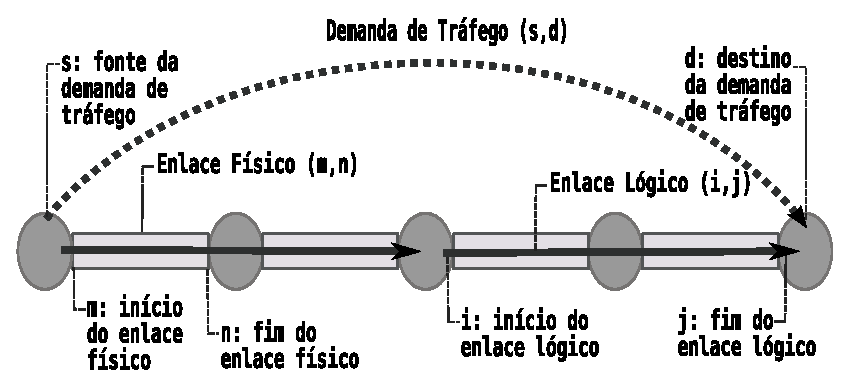
\includegraphics[bb=43 653 523 825,scale=.9]{figs/indices.eps}
\caption{Representa��o gr�fica da nota��o associada aos n�s da rede.}
\label{fig:Indices}
\end{figure}

A Figura \ref{fig:Indices} ilustra os diferentes escopos dos �ndices associados aos n�s da rede, com rela��o �s liga��es f�sicas $(m,n)$, liga��es l�gicas
$(i,j)$ e demandas de tr�fego $(s,d)$. Esta nota��o segue a conven��o comumente utilizada em trabalhos anteriores \cite{mukherjee,ram02}. �
importante dizer que esta modelagem suporta m�ltiplas liga��es f�sicas e l�gicas entre cada par de n�s, portanto, os pares $(m,n)$ e $(i,j)$ representam
conjuntos de poss�veis liga��es f�sicas e l�gicas, respectivamente. Esses conjuntos n�o ser�o explicitamente controlados, sendo esse um dos motivos
da simplicidade do modelo.

\begin{dados}
\label{Cons}
Uma inst�ncia para o modelo TWA � definida por:

\begin{enumerate}
\item $N$ $=$ N�mero de n�s da rede.
\item $W$ $=$ M�ximo de comprimentos de onda em uma liga��o f�sica.
% \item $H$ $=$ Grau f�sico m�ximo de entrada e sa�da de cada n�.
\item $K$ $=$ M�xima multiplicidade de liga��es f�sicas entre cada par $(m,n)$.
\item $Cap$ $=$ Capacidade de tr�fego de cada liga��o l�gica.
\item $C_{mn}$ $=$ Custo de uma liga��o f�sica entre o par $(m,n)$.
\item $T$ $=$ Custo por unidade de fluxo.
\item $P_{sd}$ $=$ Demanda de tr�fego, com origem $s$ e destino $d$.
\item $A_s = \sum_d P_{sd} =$ Tr�fego agregado pela origem $s$. 
\item $Q_{sd}=P_{sd}/A_s =$ Fra��o de $A_s$ correspondente � Demanda de tr�fego $P_{sd}$.
\end{enumerate}
\end{dados}

% \clearpage

 \subsection{Componentes Topol�gicos}
% \label{Top}

A vari�vel central do modelo, a partir da qual todas as demais ser�o definidas, chamada de componente topol�gico, � representada graficamente na Figura
\ref{fig:B} e formalmente definida na Vari�vel \ref{comp}. Ela sozinha representa as topologias l�gica e f�sica, as rotas f�sicas das 
liga��es l�gicas e os comprimentos de onda utilizados.

\begin{var}
\label{comp}
 Seja $B_{iw}^{mn} = k\in \{0,..,K\}$, com $i\neq n$, um componente do conjunto das liga��es l�gicas com origem $i$ e comprimento de onda $w$,
que utilizam $k$ liga��es f�sicas entre os n�s $m$ e $n$.
\end{var}

\begin{figure}[hbt]
 \centering
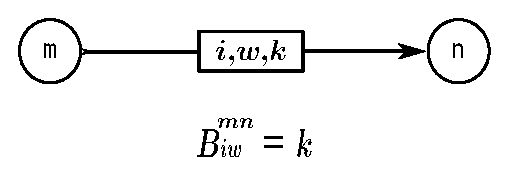
\includegraphics[bb=177 683 405 753, scale=0.9]{figs/B.eps}
% B.eps: 1179666x1179666 pixel, 300dpi, 9987.84x9987.84 cm, bb=36 739 246 805
 \caption{Representa��o gr�fica de um componente topol�gico.}
 \label{fig:B}
\end{figure}

Considerando que $B_{iw}^{mn}=k$ para algum $k \in \{0,..,K\}$, existem $k$ liga��es l�gicas originadas em $i$ no comprimento de onda $w$, passando
por $k$ liga��es f�sicas distintas entre o par de n�s $(m,n)$.  Conforme a terminologia utilizada
neste trabalho daqui por diante, \textit{um componente topol�gico $B_{iw}^{mn} = k$ � iniciado em $m$, incidente em $n$, com origem $i$,
comprimento de onda $w$ e valor $k$}.

Se $k>1$, ent�o h� multiplicidade de liga��es f�sicas entre o par de n�s $(m,n)$,
pois haveria interfer�ncia se houvessem duas liga��es l�gicas se propagando na mesma liga��o f�sica, com o mesmo comprimento de onda. Note
que $K$ limita apenas a multiplicidade das liga��es f�sicas, pois se $K=1$, $B_{iw}^{mn}$ se torna uma vari�vel bin�ria, mas ainda podem haver m�ltiplas
liga��es l�gicas entre um par $(i,j)$, utilizando rotas f�sicas distintas, ou ainda, comprimentos de onda diferentes em uma mesma
rota f�sica. Se $B_{iw}^{mn}=0$, $\forall\,(i,w)$, ent�o nenhuma liga��o f�sica entre o par de n�s $(m,n)$ � utilizada.

 Na Figura \ref{fig:Tops}, temos um exemplo de interpreta��o dos componentes topol�gicos, todos com origem no n� $v_1$ e com o 
mesmo comprimento de onda $w_1$. No item $d)$ desta figura, o valor $2$ do componente que liga os n�s $(v_1,v_2)$ � interpretado 
como duas liga��es f�sicas entre esses n�s, representadas no item $a)$. No item $b)$, vemos uma liga��o l�gica dupla entre os 
n�s $(v_1,v_3)$, onde uma delas passa de forma transparente pelo n� $v_2$, como indicado no item $c)$. Note ainda que, no item 
$d)$, h� dois caminhos l�gicos incidentes em $v_2$ mas apenas um iniciando. Isso indica que uma liga��o l�gica termina em $v_2$, 
enquanto a outra segue adiante.

% \clearpage
\begin{figure}[hbt]
 \centering
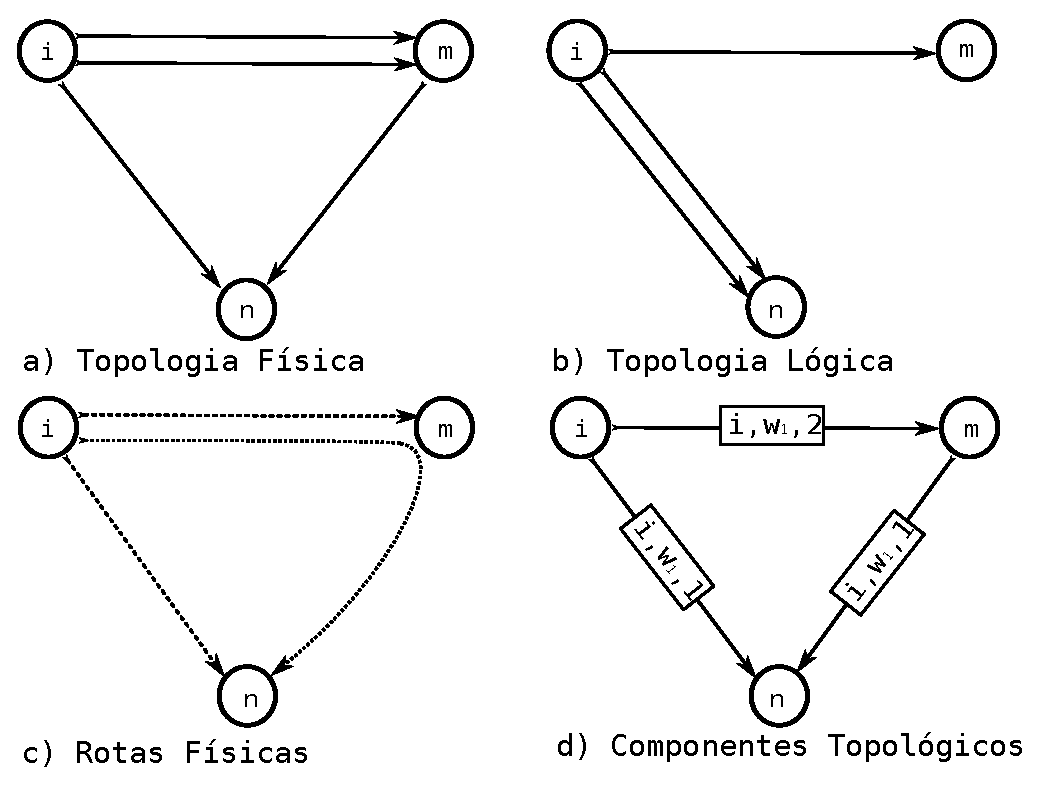
\includegraphics[width=0.8\textwidth]{figs/topologias-twa.eps}
% 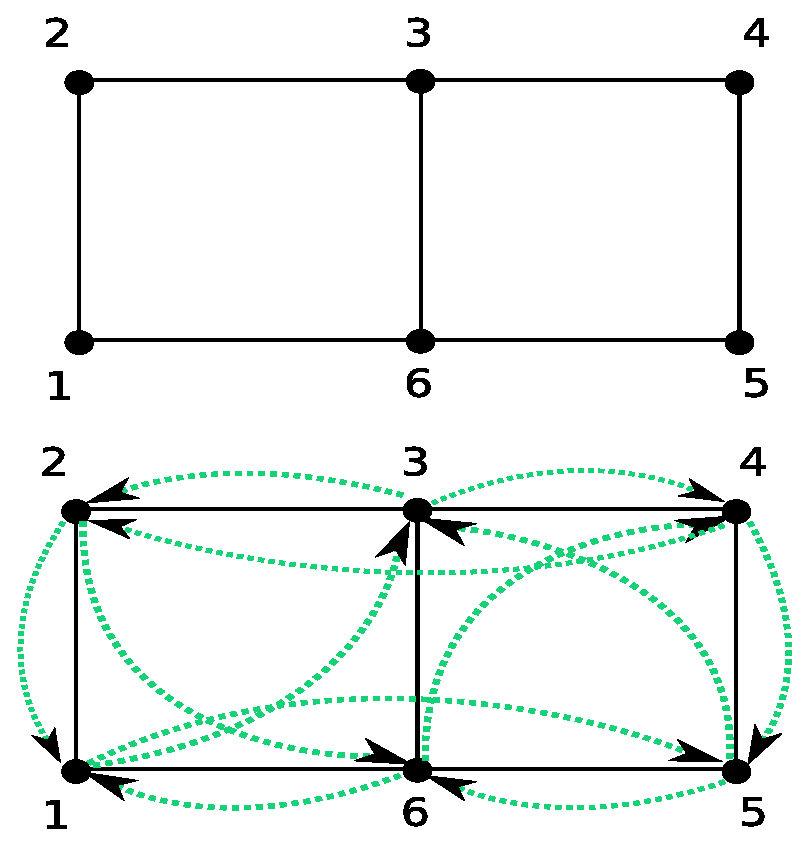
\includegraphics[bb=39 455 511 811, scale=0.4]{figs/topologias.eps}
 % topologias.eps: 1179666x1179666 pixel, 300dpi, 9987.84x9987.84 cm, bb=30 375 511 801
 \caption{Exemplo da interpreta��o dos componentes topol�gicos.}
 \label{fig:Tops}
\end{figure}
% \clearpage

A indexa��o atribu�da �s vari�veis $B_{iw}^{mn}$ especificam apenas o n� $i$ onde se iniciam as liga��es l�gicas representadas, sem deixar claro
aonde elas terminam. Isto significa que estas vari�veis agregam todas as liga��es l�gicas originadas em $i$ com comprimento de onda $w$, que utilizam as
liga��es f�sicas entre o par $(m,n)$, independente do n� $j$ em que terminam estas liga��es l�gicas. Esta t�cnica consiste em uma abordagem bastante
conhecida para a representa��o de vari�veis em problemas de distribui��o de fluxo em redes. Em \cite{Tornatore07}, este conceito de agrega��o de tr�fego �
aplicado como meio de simplifica��o do modelo, reduzindo substancialmente o n�mero de vari�veis dos problemas resultantes. No TWA, esta agrega��o cumpre o
mesmo papel de simplifica��o, cabendo �s restri��es do modelo garantir implicitamente a termina��o correta destas liga��es l�gicas agregadas nas vari�veis
$B_{iw}^{mn}$.

Para fins de compara��o entre modelos de programa��o inteira, usualmente uma vari�vel que pode assumir $K$
valores diferentes � convertida em $K$ vari�veis bin�rias \cite{cormen02}. A princ�pio, o n�mero de vari�veis bin�rias associadas aos componentes
topol�gicos seria $N^3\cdotp W\cdotp K$ \cite{cormen02}, mas devemos excluir algumas que s�o trivialmente nulas: aquelas com $i=n$, pois $i$ n�o pode ser
origem da liga��o l�gica e ao mesmo tempo destino da liga��o f�sica ($n$). Isso resulta em $N^3\cdotp W\cdotp K - N^2\cdotp K$.


\subsection{Fra��o de Fluxo das Demandas de Tr�fego}
\label{cap:twa-sec:VarFracFlow}

Para resolver o sub-problema de roteamento de tr�fego, � definida a vari�vel Vari�vel \ref{FlowVar}, que modela a fra��o de fluxo agregado para as
demandas de tr�fego. Elas s�o
semelhantes �s vari�veis de fluxo agregado utilizadas em \cite{ram96}, todavia h� duas diferen�as. Uma delas � que aqui essas vari�veis s�o normalizadas em
fun��o do tr�fego agregado na origem ($A_s$), e s�o portanto uma fra��o deste. Essa modifica��o n�o � requerida pela modelagem, tendo apenas a fun��o de
facilitar a compreens�o das restri��es do modelo, que ficam menos dependentes do dados de entrada. 

A outra diferen�a � que o fluxo � separado por comprimento de onda, como se fossem $W$ redes sem multiplexa��o sobrepostas. Isso facilita a interpreta��o
das
restri��es do modelo, e tamb�m ajuda a mant�-lo mais simples. De fato, o controle da distribui��o de fluxo deve ser feito em cada liga��o l�gica
\cite{ram02}, mas a restri��o de continuidade de comprimentos de onda exige uma equa��o para cada $w$ separadamente \cite{Zang00}. Soma-se a isso o fato de
que nesta modelagem m�ltiplas liga��es l�gicas s�o agregadas em cada par $(i,j)$ para todos os valores $w$ utilizados. Assim, separando o tr�fego por
comprimento de onda, foi poss�vel combinar o controle da distribui��o de tr�fego com a restri��o de continuidade de comprimentos de onda. Isso ser� tratado
com mais detalhes na Se��o \ref{cap:twa-sec:Bconserv_Cap}.

\begin{var}
 \label{FlowVar}
 Seja $q_{sw}^{ij} \in [0,1]$ a fra��o do fluxo originado em $s$, passando pelas liga��es l�gicas entre o par $(i,j)$ com comprimento de onda $w$,
onde $s\neq j$. 
\end{var}

Tamb�m devem ser exclu�das do modelo, por serem trivialmente nulas, as fra��es de fluxo com $s=j$. Pois $j$ � destino do tr�fego, n�o podendo ser ao mesmo
tempo origem ($s$). Assim, o n�mero de vari�veis reais associadas �s fra��es de fluxo � $N^3\cdotp W - N^2$.

\subsection{Topologia F�sica}
\label{cap:twa-sec:VarFis}

Apesar da topologia f�sica ser determinada pelos componentes topol�gicos, para fins de controle do custo de instala��o da rede f�sica,
s�o necess�rias novas inc�gnitas. Para este fim, � definida a Vari�vel \ref{FisVar}, que registrar� em $D_{mn}$ a multiplicidade f�sica determinada pelos
componentes topol�gicos. Se $D_{mn}=0$, n�o h� liga��es f�sicas entre o par $(m,n)$, mas se $D_{mn}=k$, para algum $k \in \{0,..,K\}$, existem $k$ liga��es
f�sicas entre o par $(m,n)$.

\begin{var}
\label{FisVar}
 Seja $D_{mn} \in \{0,..,K\}$ o n�mero de liga��es f�sicas entre o par de n�s $(m,n)$. 
\end{var}

O n�mero de vari�veis bin�rias associadas � $D_{mn}$ �  $N^2\cdotp K - N\cdotp K$ \cite{cormen02}, pois deve-se desconsiderar as vari�veis onde $m=n$. 

 \section{Custo de instala��o e Opera��o}
 \label{cap:twa-sec:funcaoobjetivo}


Duas m�tricas importantes no projeto da redes �pticas s�o os custos de instala��o e opera��o \cite{mukherjee}. 
O custo de instala��o $C_{mn}$ � o custo associado a uma liga��o f�sica entre o par de n�s $(m,n)$. O custo total de instala��o � dado na equa��o
\ref{eq:custoInstlacao}. O custo de opera��o $TO$, definido como o custo por unidade de fluxo, � calculado na equa��o \ref{eq:CustoDeOperacao}, e
influencia tamb�m no dimensionamento dos n�s da rede.

\begin{equation}
   CI = \sum_{mn} C_{mn}\cdot D_{mn}
   \label{eq:custoInstlacao}
\end{equation}


\begin{equation}
    TO = \sum_{sijw} T\cdot q_{sw}^{ij}\cdot A_s
    \label{eq:CustoDeOperacao}
\end{equation}

O custo de opera��o pode ser dividido em duas partes: uma constante, formada pelas demandas de tr�fego (equa��o \ref{eq:Tc}), que necessariamente
dever�o ser roteadas; e outra vari�vel, composta pelo tr�fego adicional que � gerado, ou seja, o tr�fego 
retransmitido (equa��o \ref{eq:Tv}). A parte constante do custo de opera��o n�o influenciaria na fun��o objetivo, por isso n�o ser� inclu�da em seu c�lculo,
dado na equa��o \ref{eq:FO}.

\begin{equation}
     TOC = \sum_{sd} T\cdot P_{sd}
   \label{eq:Tc}
\end{equation}

\begin{equation}
     TOV = \sum_{sijw} T\cdot q_{sw}^{ij}\cdot A_s\,,\quad \mbox{\small$i\neq s$}
   \label{eq:Tv}
\end{equation}

\begin{equation}
   FO = CI + TOC
   \label{eq:FO}
\end{equation}

Outro ponto positivo dessas m�tricas � que minimizar o custo por unidade de fluxo � equivalente a minimizar o tr�fego retransmitido na rede, o que por 
sua vez, equivale a minimizar o processamento eletr�nico de tr�fego dos n�s da rede \cite{Renato06}. Al�m disso, ser� necess�ria nesta modelagem uma
restri��o de limita��o da capacidade das liga��es l�gicas ($Cap$), que equivale � limitar o congestionamento na rede. Assim, limitando a capacidade e
minimizando o custo de opera��o, temos uma abordagem eficiente, quanto ao custo 
computacional, para controlar tamb�m o congestionamento e o processamento, importantes m�tricas no projeto da topologia virtual \cite{Renato06,ram02}. 

Se n�o for necess�rio ponderar o custo por unidade de fluxo, basta fazer $T=1$, e se n�o for necess�rio considerar o custo 
total de instala��o ($CI$), basta fazer $C_{mn}=0$ para todo $(m,n)$. Deste modo seria 
simplesmente um modelo de minimiza��o do processamento, com limita��o do congestionamento \cite{Renato06}. 


 \section{O Modelo TWA}
 
 Nesta se��o � apresentada a forma b�sica do modelo TWA. Suas restri��es s�o apresentadas a seguir, ap�s a fun��o objetivo apresentada na se��o anterior.

\textbf{Fun��o Objetivo}


\begin{itemize}

\item Minimizar o Custo de Instala��o e Opera��o:

\begin{equation}
 \sum_{mn} C_{mn}\cdot D_{mn} + \sum_{sijw} T\cdot q_{sw}^{ij}\cdot A_s \,,\quad \mbox{\small$i\neq s$}
\label{fo:MinC}
\end{equation}

\end{itemize}

\textbf{Restri��es}

\begin{itemize}
 \item Restri��o de Continuidade de Comprimentos de Onda e Limita��o de Capacidade:

\begin{equation}
\sum_{s} q_{sw}^{iv}\cdot A_s \leqslant Cap\cdot \left(\sum_{m} B_{iw}^{mv} - \sum_{n} B_{iw}^{vn}\right) \Forall{(i,v,w)} \mbox{, com $i\neq v$}
\label{rest:DefCapFlow}
\end{equation} 

\item Topologia F�sica:

\begin{equation}
\sum_i B_{iw}^{mn} \leqslant D_{mn} \Forall{(m,n,w)}
\label{rest:DefFis}
\end{equation} 

\item Conserva��o de Fluxo:

\begin{equation}
\sum_{jw} q_{vw}^{vj} = 1 \Forall{v} 
\label{rest:ConservFlowOut}
\end{equation} 
 
\begin{equation}
\sum_{iw} q_{sw}^{iv} - \sum_{jw} q_{sw}^{vj} = Q_{sv} \Forall{(s,v)} \mbox{, com $s\neq v$}
\label{rest:ConservFlow}
\end{equation}
 
\end{itemize}

O n�mero de equa��es no modelo b�sico � $ 2\cdot N^2\cdot W + N^2 + N $, que em nota��o assint�tica � $\Theta(N^2\cdot W)$ \cite{cormen02}. Somando o
n�mero vari�veis bin�rias associadas aos componentes topol�gicos, mais as associadas � topologia f�sica, temos $\Theta(N^3\cdotp
W\cdotp K)$. Portanto, em n�mero de vari�veis e restri��es, o TWA � similar a modelos eficientes, mas que resolvem
apenas o sub-problema RWA, como os que foram estudados em \cite{Jaumard04}. Na Tabela \ref{tab:num_var} s�o resumidos os dados sobre n�mero de
vari�veis e equa��es.

\begin{table}[htb]
{%
\newcommand{\mc}[3]{\multicolumn{#1}{#2}{#3}}
\begin{center}
\begin{tabular}{lll}\hline
\mc{1}{|l|}{Bin�rias} & \mc{1}{l|}{Reais} & \mc{1}{c|}{Equa��es}\\\hline
\mc{1}{|l|}{$\Theta(N^3\cdotp W\cdotp K)$} & \mc{1}{|l|}{$\Theta(N^3\cdot W)$} & \mc{1}{|l|}{$\Theta(N^2\cdot W)$}\\\hline
\end{tabular}
\end{center}
}%
\caption{Numero de vari�veis bin�rias, reais e equa��es no TWA.}
\label{tab:num_var}
\end{table}



\subsection{Planos L�gicos}
\label{cap:twa-sec:planos}

Como os componentes topol�gicos e as fra��es de fluxo s�o indexados pelo comprimento de onda, a distribui��o tr�fego � feita em partes disjuntas da
topologia l�gica, tamb�m separadas por comprimento de onda. De fato, esta modelagem � focada nas rotas f�sicas; elas � que definem as topologias l�gica e
f�sica. Pode-se separar as rotas e seu respectivo tr�fego em partes disjuntas da rede, agrupadas por cada valor de $w$. Essas rotas n�o compartilham as
mesmas liga��es f�sicas pois todas possuem o mesmo comprimento de onda. Todavia podem n�o ser disjuntas pois ainda � poss�vel que passem por um mesmo n�
intermedi�rio.

Mas essa separa��o s� ocorre na
topologia l�gica, pois cada rota corresponde a uma liga��o l�gica. Na topologia f�sica, duas rotas podem compartilhar uma mesma liga��o f�sica utilizando
comprimentos de onda diferentes.

Na Figura \ref{fig:planos_logicos} � representada a separa��o da topologia l�gica por
comprimentos de onda. Essas por��es disjuntas s�o vistas na figura como planos paralelos que, quando sobrepostos, formam a topologia
l�gica. Esses planos ser�o aqui chamados de planos l�gicos, cada um associado a um comprimento de onda, onde um par $(i,j)$ pode ainda representar m�ltiplas
liga��es l�gicas utilizando um mesmo $w$. 

\begin{figure}[htb]
	\centering
	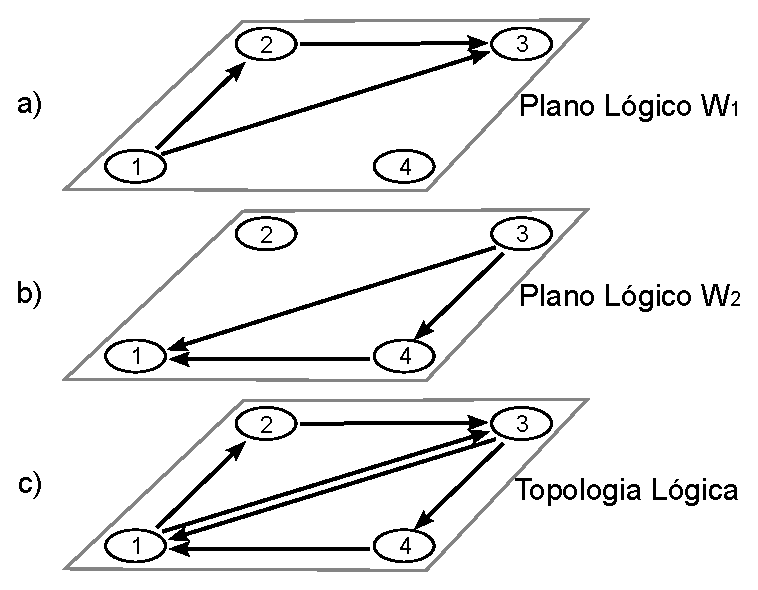
\includegraphics[bb=152 525 500 792,scale=0.7]{./figs/planos_logicos.eps}
	% planos_logicos.eps: 0x0 pixel, 300dpi, 0.00x0.00 cm, bb=152 524 442 792
	\caption{Esquema da separa��o da topologia l�gica por comprimento de onda.}
	\label{fig:planos_logicos}
\end{figure}

Essa forma de visualizar a topologia l�gica tem apenas a finalidade de facilitar a interpreta��o das restri��es,
pois permite ver o projeto como se fossem $W$ redes sem multiplexa��o sobrepostas.
Nas se��es que se seguem no restante deste cap�tulo, a separa��o da topologia l�gica por comprimento de onda ser� usada na explana��o sobre as restri��es do
modelo TWA.  

\subsection{Continuidade de Comprimentos de Onda e Capacidade}
\label{cap:twa-sec:Bconserv_Cap}

A Restri��o \ref{rest:DefCapFlow} acumula m�ltiplas fun��es, atuando como restri��o de continuidade de comprimentos de onda e limita��o de
capacidade. Em cada plano l�gico $w$, ela garante a continuidade das rotas f�sicas, onde os componentes topol�gicos devem formar uma caminho sobre a
topologia f�sica, conservando o mesmo comprimento de onda. Esses percursos n�o s�o controlados explicitamente; eles s�o garantidos pela conserva��o dos
componentes topol�gicos nos n�s intermedi�rios, semelhante a uma restri��o de conserva��o de fluxo \cite{ramamurthy99}. 

A Restri��o \ref{rest:DefCapFlow} � repetida na equa��o \ref{eq:DefCapFlow} para facilitar a leitura desta se��o. Nela, a conserva��o dos percursos l�gicos
� feita da seguinte forma: a soma dos componentes das liga��es l�gicas iniciadas em um n� $i$ no plano $w$, partindo de um n� intermedi�rio $v$, deve ser
menor ou igual � quantidade recebida. Isso � garantido se a equa��o \ref{eq:ConserB} for satisfeita.

\begin{equation}
\sum_{s} q_{sw}^{iv}\cdot A_s \leqslant Cap\cdot \left(\sum_{m} B_{iw}^{mv} - \sum_{n} B_{iw}^{vn}\right) \Forall{(i,v,w)} \mbox{, com $i\neq v$}
\label{eq:DefCapFlow}
\end{equation} 

\begin{equation}
   \sum_{n} B_{iw}^{vn} \leqslant \sum_{m} B_{iw}^{mv}  \Forall{(i,v,w)}
   \label{eq:ConserB}
\end{equation}

A equa��o \ref{eq:ConserB} pode ser reescrita na forma da equa��o \ref{eq:ConserBdif}, que define $LL^{iv}_w$, a diferen�a entre a soma dos
componentes chegando e saindo de $v$, originados em $i$ no plano $w$. O valor
$LL^{iv}_w$ representa a quantidade de liga��es l�gicas que n�o t�m continuidade ao passar por $v$, ou seja, s�o as liga��es l�gicas incidentes em $v$,
com origem em $i$ no plano $w$.

\begin{equation}
  LL^{iv}_w = \sum_{m} B_{iw}^{mv} - \sum_{n} B_{iw}^{vn} \geqslant 0 \Forall{(i,v,w)}
   \label{eq:ConserBdif}
\end{equation}

 Por sua vez, a equa��o \ref{eq:ConserBdif} � equivalente � equa��o
\ref{eq:ConserBcap}. Este �ltima � garantida pela Restri��o \ref{rest:DefCapFlow}, como fica demostrado pela equa��o \ref{eq:ConserBfim}, pois tomando-a
como premissa conclui-se a equa��o \ref{eq:ConserBcap}. Portanto, a equa��o \ref{eq:ConserB} � v�lida. 

\begin{equation}
   0  \leqslant Cap\cdot LL^{iv}_w \Forall{(i,v,w)}
   \label{eq:ConserBcap}
\end{equation}

\begin{equation}
   \sum_{s} q_{sw}^{iv}\cdot A_s  \leqslant Cap\cdot LL^{iv}_w \Forall{(i,v,w)}
   \label{eq:ConserBfim}
\end{equation}

Na figura \ref{fig:Bconserv} � ilustrada a forma como a conserva��o dos percursos l�gicos � feita. Nela v�-se dois componentes chegando no
n� intermedi�rio $v$, ambos comp�em liga��es l�gicas no plano $w$ iniciadas no n� $i$, que n�o est� representado na figura, igualmente ao componente que
deixa $v$. A soma dos valores dos componentes que chegam � $3$ e a dos que saem � $2$, portanto a conserva��o est� mantida. Neste exemplo, como h�
diferen�a de $1$ entre a quantidade de componentes chegando e saindo de $v$, ent�o, necessariamente h� $1$ liga��o l�gica terminando em $v$; para a qual
ele deixa de ser visto como um n� intermedi�rio, se tornando o destino dessa liga��o l�gica. A conserva��o n�o seria mantida no plano $w$ houvessem
componentes partindo de $v$ em maior quantidade do que chegando, pois ai n�o haveria rastreabilidade do percurso at� sua origem $i$. 
 
\begin{figure}[htb]
	\centering
	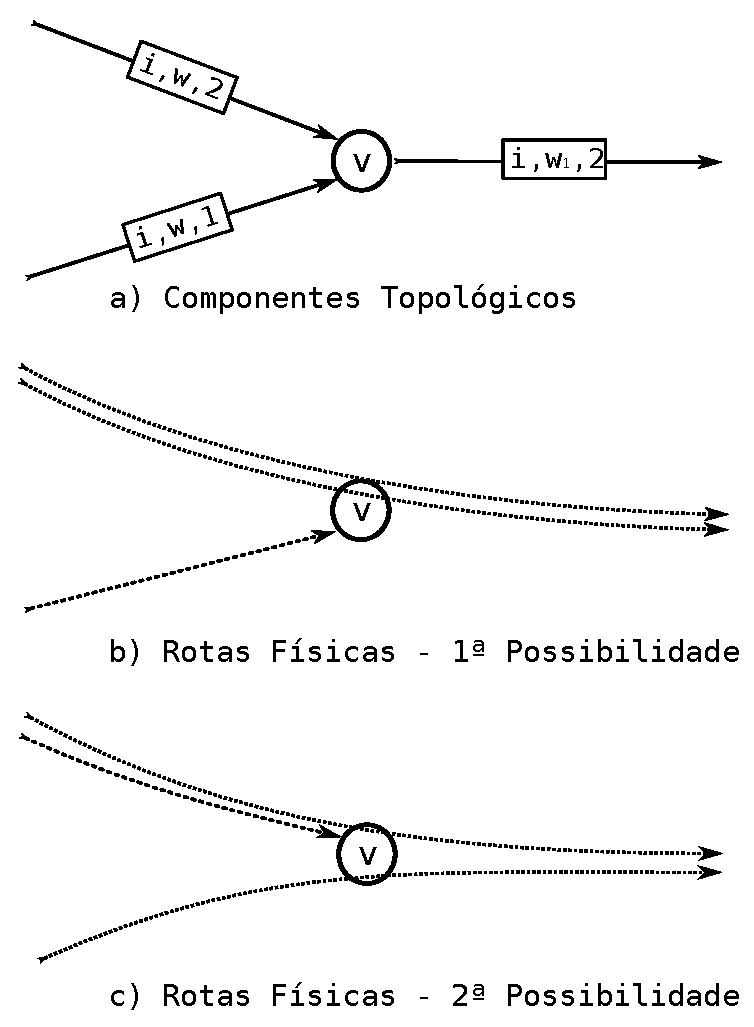
\includegraphics[bb=109 621 445 749,scale=0.7]{./figs/B_conserv.eps}
	% B_conserv.eps: 0x0 pixel, 300dpi, 0.00x0.00 cm, bb=106 272 452 749
	\caption{Conserva��o dos Percursos L�gicos.}
	\label{fig:Bconserv}
\end{figure}

A Restri��o \ref{rest:DefCapFlow} � um conjunto de equa��es, onde cada uma trata de um par $(i,j)$ em um plano l�gico $w$. Portanto, a capacidade das
liga��es l�gicas associadas ao par $(i,j)$ � a capacidade de cada uma ($Cap$) multiplicada pelo n�mero de liga��es l�gicas entre $(i,j)$ no plano l�gico
$w$.
Este segundo fator � $LL^{ij}_w$, calculado na equa��o \ref{eq:ConserBdif}. Todo o tr�fego passando pelas liga��es l�gicas $(i,j)$ nesse plano
deve ser limitado por $Cap\cdot
LL^{ij}_w$, o que de fato � feito pela Restri��o \ref{rest:DefCapFlow}. 

A Restri��o \ref{rest:DefCapFlow} ainda acumula uma fun��o que, por ser intuitiva, pode passar desapercebida, mas � fundamental para a consist�ncia do
modelo. Ela anula as fra��es de fluxo agregado entre os n�s n�o conectados diretamente por liga��es l�gicas. Quando $LL^{ij}_w = 0$, ou seja, n�o
h� liga��es l�gicas entre o par $(i,j)$ no plano $w$, as fra��es de fluxo $q_{sw}^{ij}$ ser�o anuladas pela Restri��o \ref{rest:DefCapFlow}, para todas as
origens $s$.

\subsection{Controle da Topologia F�sica}

Com a finalidade de controlar pela fun��o objetivo \ref{fo:MinC} a quantidade de liga��es f�sicas definidas pelos componentes topol�gicos, a Restri��o
\ref{rest:DefFis} acumula nas vari�veis $D_{mn}$ a multiplicidade determinada pelos componentes. Ela � repetida na
equa��o \ref{eq:DefFis} para facilitar a leitura desta se��o. Dado um par $(m,n)$, as equa��es
dessa restri��o s�o ainda separadas por comprimento de onda. Pois se todos os componentes topol�gicos alocados em $(m,n)$ usarem o mesmo $w$, apenas uma
liga��o f�sica ser� necess�ria. Se usarem comprimentos de onda diferentes, $D_{mn}$ precisar� atender ao maior desses componentes topol�gicos. Portanto, a
restri��o \ref{rest:DefFis}, minimiza a soma dos maiores de componentes topol�gicos em cada par $(m,n)$, por for�a do fator $CI$ na fun��o objetivo (Se��o
\ref{cap:twa-sec:funcaoobjetivo}).

\begin{equation}
\sum_i B_{iw}^{mn} \leqslant D_{mn} \Forall{(m,n,w)}
\label{eq:DefFis}
\end{equation} 

\begin{figure}[htb]
	\centering
	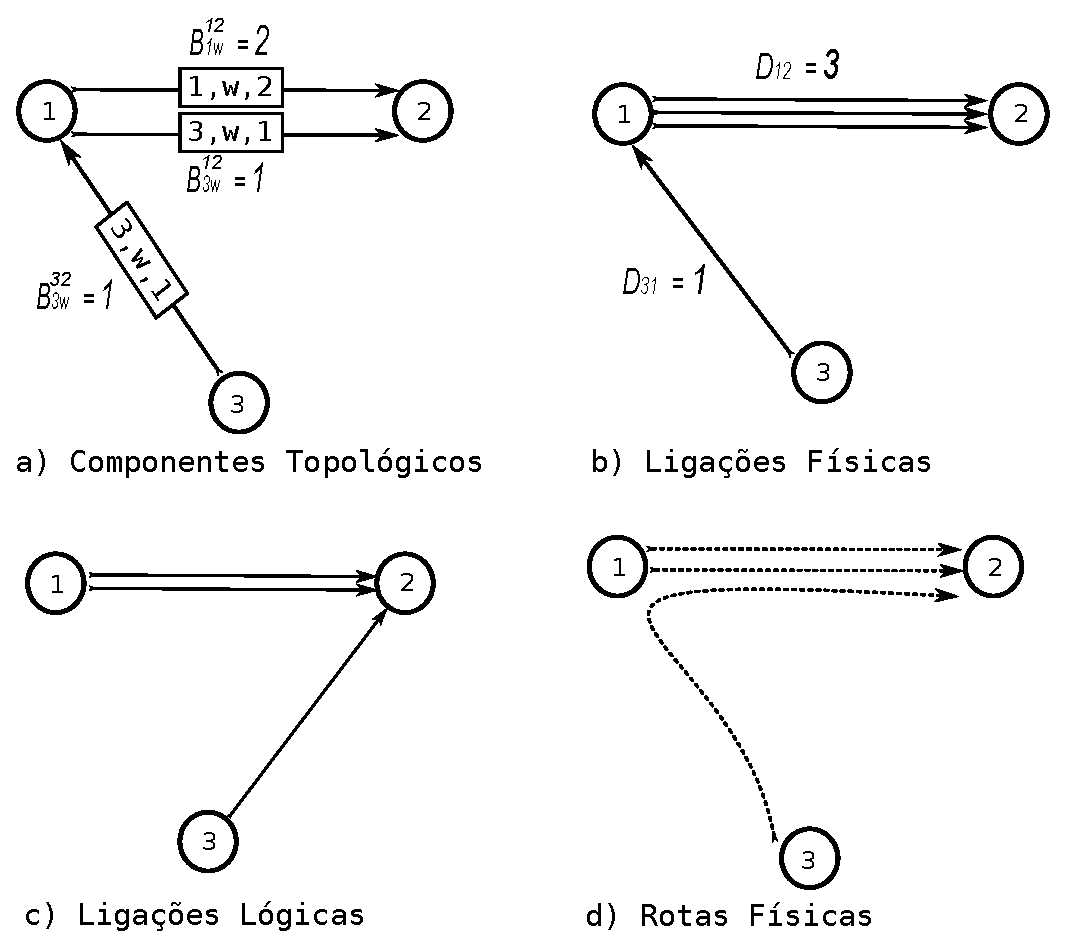
\includegraphics[bb=37 371 534 812, scale=0.7]{./figs/Var_Dmn.eps}
	% Var_Dmn.eps: 0x0 pixel, 300dpi, 0.00x0.00 cm, bb=34 593 536 800
	\caption{Interpreta��o dos componentes topol�gicos na vari�vel $D_{mn}$.}
	\label{fig:varDmn}
\end{figure}

Na Figura \ref{fig:varDmn} est� um exemplo de interpreta��o dos componentes topol�gicos na vari�vel $D_{mn}$. No item $a$ est�o os componentes topol�gicos
que definem as liga��es f�sicas indicadas no item $b$. Nos itens $c$ e $d$ est�o as liga��es l�gicas e as rotas f�sicas correspondentes.

\subsection{Conserva��o de Fluxo}

A conserva��o de fluxo � assegurada pelas Restri��es \ref{rest:ConservFlowOut} e \ref{rest:ConservFlow}, que tamb�m garantem o envio e a entrega das
demandas de tr�fego. Elas s�o repetidas nas equa��es \ref{eq:ConservFlowOut} e \ref{eq:ConservFlow} para facilitar a leitura desta se��o.  
Essas restri��es s�o semelhantes �s encontradas na modelagem agregada para o VTD \cite{ram02}. Al�m da separa��o do tr�fego por
comprimento de onda e da normaliza��o das vari�veis, como foi comentado na Se��o \ref{cap:twa-sec:VarFracFlow}, a interpreta��o das restri��es �
sutilmente diferente pois um par $(i,j)$ representa um conjunto de liga��es l�gicas. 

\begin{equation}
\sum_{jw} q_{vw}^{vj} = 1 \Forall{v} 
\label{eq:ConservFlowOut}
\end{equation} 
 
\begin{equation}
\sum_{iw} q_{sw}^{iv} - \sum_{jw} q_{sw}^{vj} = Q_{sv} \Forall{(s,v)} \mbox{, com $s\neq v$}
\label{eq:ConservFlow}
\end{equation}

Cada par $(i,j)$ � visto nas restri��es de controle de fluxo como um �nico caminho, unindo todos os planos l�gicos. Se o par representar na verdade
m�ltiplas
liga��es l�gicas, a diferen�a � que ele ter� uma capacidade maior de receber tr�fego, que � controlada pela Restri��o \ref{rest:DefCapFlow}. Deste modo,
essas restri��es funcionam da mesma forma que em \cite{ram96}. Portanto, s�o as restri��es de conserva��o de fluxo que fazem a correla��o ente os planos
l�gicos.

A Restri��o \ref{rest:ConservFlowOut} garante que todo o tr�fego originado em cada n� $v$ seja emitido para a rede, exigindo que a soma das fra��es
de tr�fego, em todos os planos l�gicos, que iniciam na origem ($i=s=v$) seja igual a $1$, ou seja, $100\%$ do tr�fego originado em $v$. 

Por sua vez, a
Restri��o \ref{rest:ConservFlow} garante que o tr�fego emitido seja encaminhado atrav�s da rede e entregue no destino. Fixada uma origem de tr�fego $s$,
para cada n� intermedi�rio $v$ ($v\neq s$) a por��o de tr�fego que deve ser entregue � $Q_{sv}$. Ela � igual � soma do tr�fego chegando por todos
os planos l�gicos $w$, vindo de qualquer n� intermedi�rio $i$, subtra�da da soma do tr�fego partindo com destino a qualquer n� $j$, em qualquer
plano $w$. O tr�fego n�o entregue em $v$ continua seguindo seu caminho pela rede at� seu destino, e deste modo � feita rastreabilidade do tr�fego at� sua
origem. Esta restri��o apenas n�o garante que o tr�fego seja emitido na origem, tarefa cumprida pela Restri��o \ref{rest:ConservFlowOut}.

O tr�fego pode ser subdividido e transportado simultaneamente por mais de uma liga��o l�gica entre o par $(i,j)$, no plano $w$. Neste caso, como as rotas
ter�o o mesmo comprimento de onda, eles n�o compartilham liga��es f�sicas ao longo do percurso. Mas essas rotas podem ainda n�o ser disjuntas, pois �
poss�vel compartilharem n�s intermedi�rios.

\section{Limita��es da Forma B�sica do TWA}

Dada a forma agregada como � feito o roteamento dos comprimentos de onda e tamb�m pela forma impl�cita do tratamento de m�ltiplas liga��es l�gicas, sem
separ�-las em vari�veis de decis�o pr�prias, algumas quest�es de menor complexidade n�o s�o decididas pelo TWA.  Na solu��o provida pelo modelo, s�o
alocados recursos suficiente para
atender ao projeto, da forma mais econ�mica poss�vel. Mas nem todos os detalhes da configura��o da rede s�o determinados.

Como ser� mostrado nesta se��o, essas omiss�es n�o
prejudicam o projeto dentro do escopo adotado. Podendo essas quest�es n�o resolvidas serem tratadas em fases posteriores do projeto a partir da solu��o
provida pelo modelo. Isso garante a simplicidade do TWA, permitindo uma modelagem com poucas restri��es e vari�veis. 

Na lista a seguir s�o enumeradas as limita��es da forma b�sica do TWA. Em seguida, cada uma ser� explicada e formas de trat�-las ser�o
sugeridas.

\begin{enumerate}
	\item Pode n�o haver uma forma �nica para configura��o das rotas f�sicas em cada plano l�gico.
	\item Podem ocorrer ciclos nas rotas f�sicas.
	\item Pode n�o ser poss�vel saber com exatid�o a dist�ncia percorrida pelo tr�fego.
	\item N�o � modelada a exata divis�o do tr�fego entre m�ltiplas liga��es l�gicas.
	\item N�o � poss�vel minimizar diretamente o congestionamento na forma b�sica do modelo.
	\item Podem haver liga��es f�sicas n�o utilizadas na solu��o.
\end{enumerate}

Como o roteamento de comprimento de onda � feito de forma agregada, podem haver mais de uma possibilidade de configura��o das rotas f�sicas em cada plano
l�gico. Na Figura \ref{fig:B_unsolved}, � mostrado um arranjo de componentes topol�gicos com duas possibilidades de interpreta��o. Necessariamente duas
liga��es l�gicas no plano $w_1$ passam transparentemente por $v_4$, enquanto uma nele termina. Ambas possibilidades de interpreta��o dos componentes s�o
v�lidas, ou seja, o TWA n�o modela o exato percurso f�sico das liga��es l�gicas em cada plano. Todavia,
isso n�o interfere na modelagem do restante do problema e n�o precisa ser resolvido nesta fase do projeto. 

De posse da solu��o provida pelo TWA, as
rotas que possu�rem alternativas de configura��o podem ser decididas levando-se em considera��o outras m�tricas n�o abordadas aqui, como por exemplo o fator
BL, que pondera tr�fego com a dist�ncia percorrida sobre a topologia f�sica \cite{Agrawal97}. Esse tratamento seria feito para cada par $(i,j)$
independente, sendo quest�es de baixa complexidade.

\begin{figure}[htb]
	\centering
	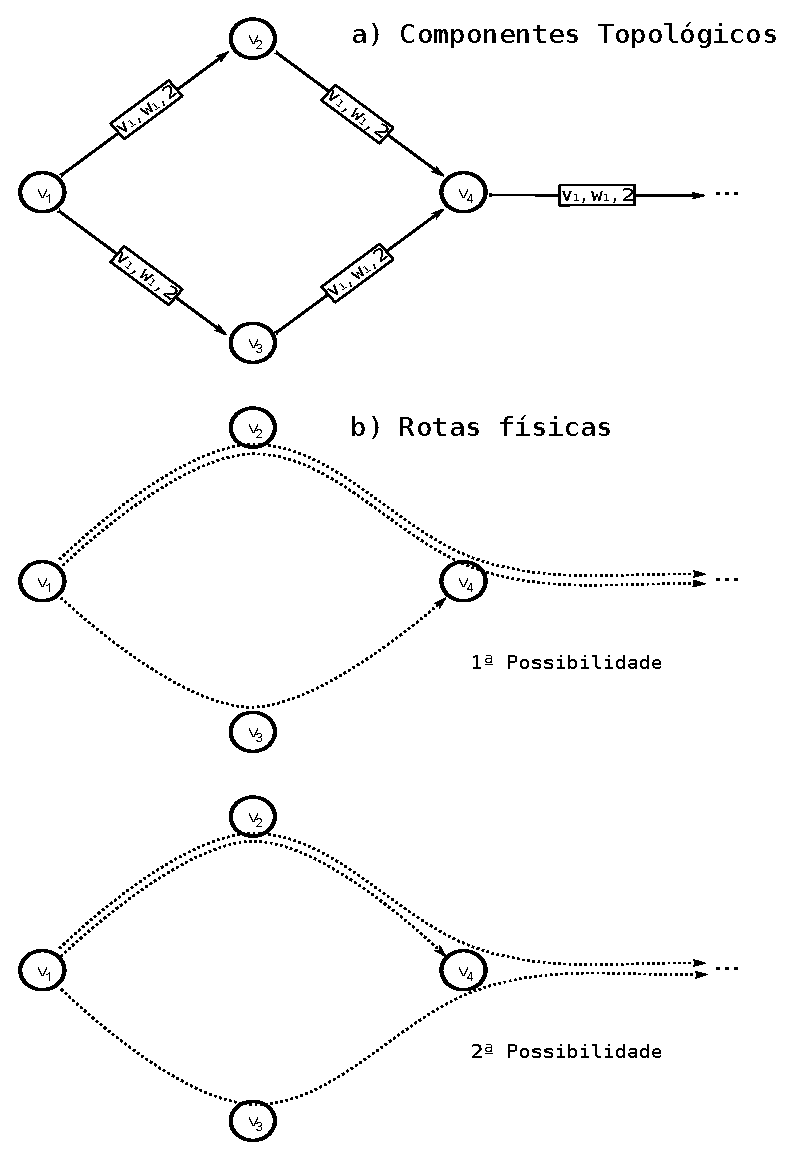
\includegraphics[bb=108 270 473 811,scale=0.7]{./figs/B_unsolved.eps}
	% B_unsolved.eps: 0x0 pixel, 300dpi, 0.00x0.00 cm, bb=108 270 473 811
	\caption{Duas possibilidades de interpreta��o dos componentes topol�gicos.}
	\label{fig:B_unsolved}
\end{figure}

Na forma b�sica do modelo TWA, podem aparecer ciclos nas rotas f�sicas, pois n�o h� esse controle no modelo b�sico. Isso poderia ser minimizado adicionando
a soma de todos os componentes topol�gicos na fun��o objetivo. Mas esses ciclos n�o interferem na modelagem e podem ser facilmente localizados e retirados
analisando a solu��o obtida.

Outra quest�o a ser determinada envolve o fato de um par $(i,j)$ poder representar m�ltiplas liga��es l�gicas. Sempre haver� banda suficiente
para atender ao tr�fego alocado respeitando � capacidade individual; isso � garantido pela Restri��o \ref{rest:DefCapFlow}. Todavia, na distribui��o do
tr�fego cada par $(i,j)$ � visto como um �nico caminho, e o tr�fego � separado apenas por comprimento de onda. O tr�fego pode ser subdividido e
transportado simultaneamente por mais de uma liga��o l�gica entre o par $(i,j)$ no plano $w$, sem compartilhar liga��es f�sicas ao longo do percurso. Mas
n�o fica definida a divis�o de tr�fego entre cada liga��o. 

A exata divis�o do tr�fego tamb�m pode ser definida em outra fase do projeto
e n�o precisa ser modelada aqui. Todavia, seria razo�vel assumir que o tr�fego fosse dividido igualmente entre as liga��es, para n�o sobrecarregar uma em
detrimento da outra. Ou poderia-se tamb�m aplicar o fator BL para fazer a divis�o do tr�fego considerando a dist�ncia percorrida. Novamente, essas
situa��es s�o pontuais, resolvendo-se para cada par $(i,j)$ individualmente sem demandar expressivo custo computacional.

Em virtude de n�o ser modelada a exata divis�o do tr�fego entre m�ltiplas liga��es l�gicas, n�o � poss�vel minimizar diretamente o
congestionamento \cite{ram02}. Mas, a capacidade das liga��es l�gicas pode exercer o papel de limitante superior (\textit{upper bound}) para o
congestionamento. Conjuntamente com a minimiza��o do tr�fego na fun��o objetivo, como foi comentado na Se��o \ref{cap:twa-sec:funcaoobjetivo}, temos uma boa
abordagem para tratar do congestionamento, como foi demostrado em \cite{Renato06}.

Por fim resta tratar da possibilidade da topologia f�sica determinada pelos componentes topol�gicos poder ser superestimada na vari�vel $D_{mn}$.
A Restri��o \ref{rest:DefFis} apenas exige que a vari�vel $D_{mn}$ seja suficiente para atender aos componentes topol�gicos, mas permite que ela assuma
valores maiores que o necess�rio. Todavia, esse poss�vel excesso n�o interfere na consist�ncia do que � modelado pelos componentes topol�gicos. Al�m disso,
ele � controlado indiretamente minimizando a fun��o objetivo, por meio do custo de instala��o, e pode ainda ser tratado analisando a solu��o fornecida,
extraindo os valores corretos diretamente dos componentes topol�gicos. A corre��o feita atrav�s da fun��o objetivo funcionaria tamb�m com qualquer outra
m�trica diretamente relacionada com a vari�vel $D_{mn}$ que fosse minimizada. 









%%%%%%%%%%%%%%%%%%%%%%%%%%%%%%%%%%%%%
%% Adapta��es do Modelo B�sico
%% Copyright 2009 Fabio de Oliveira Lima.
%% Este documento � distribu�do nos termos da licen�a 
%% GNU General Public License v2.
%%%%%%%%%%%%%%%%%%%%%%%%%%%%%%%%%%%%%


\chapter{Extens�es ao Modelo B�sico}
\label{cases}

Neste cap�tulo s�o apresentados outros casos de uso da modelagem TWA. Dada a abrang�ncia da modelagem diversas m�tricas podem ser controladas ou
diretamente minimizadas, conforme a aplica��o. Apresentamos agora como podem ser inclu�dos par�metros de controle bem conhecidos, sendo que alguns deles
ser�o utilizados
nos experimentos computacionais das Se��es \ref{cap:testes-sec:karcius} e \ref{cap:testes-sec:sivarajan}.


Veremos, por exemplo, como incluir as restri��es de controle do grau l�gico dos n�s e como usar o congestionamento como fun��o objetivo, duas considera��es
comuns das modelagens de VTD \cite{ram02}. Ser�o mostradas tamb�m formas de controlar ou otimizar o n�mero de comprimentos de onda, entre outras m�tricas
normalmente vistas em modelos de RWA
\cite{Zang00}.

% Algumas vezes ao longo desta se��o ser� necess�rio considerar a capacidade f�sica do n� $m$ de realizar liga��es l�gicas 
% (Dados \ref{CapLogi}), que � a capacidade do \textit{Optical switch} de receber ou originar liga��es \cite{Zang00}. 
% 
% \zz
% \begin{dados}
% Se a topologia f�sica � uma vari�vel do modelo ($D_{mn}$), o grau f�sico de entrada e sa�da $H$ � considerado uniforme para 
% a rede e $CapLog_m = H\cdot W$. Caso seja de interesse fixar a topologia f�sica, passando a mesma como par�metro do modelo, 
% $CapLog_m = \sum_n D_{m,n}\cdot W$.\label{CapLogi}
% \end{dados}

\section{Topologia F�sica}

Se a vari�vel de topologia f�sica $D_{m,n}$ n�o for minimizada direta ou indiretamente na fun��o objetivo, pode-se usar a equa��o
\ref{eq:CtrlFis} para anular as liga��es f�sicas n�o utilizadas. Entretanto, quando houverem liga��es f�sicas utilizadas entre o par $(m,n)$
ainda seria poss�vel que $D_{mn}$ registre valores maiores que o necess�rio para atender aos componentes topol�gicos, conforme foi comentado na Se��o
\ref{cap:twa-sec:limitacoes} a respeito da Restri��o \ref{rest:DefFis}. Para facilitar o a leitura da se��o a Restri��o \ref{rest:DefFis} � repetida na
equa��o \ref{eq:cases:DefFis}. Mas, se $D_{mn}$ n�o influencia na fun��o objetivo, esse excesso poder� ser retirado analizando a solu��o obtida.

\begin{equation}
	\sum_{i,w} B_{iw}^{mn} \geqslant D_{mn} \Forall{(m,n)}
	\label{eq:CtrlFis}
\end{equation}

\begin{equation}
\sum_i B_{iw}^{mn} \leqslant D_{mn} \Forall{(m,n,w)}
\label{eq:cases:DefFis}
\end{equation} 

A topologia f�sica pode ser um dos dados de entrada do problema, fixando em $D_{mn}$ os valores da rede existente.
Neste caso, a fun��o da restri��o de controle da topologia f�sica no modelo b�sico (\ref{rest:DefFis}) seria limitar a multiplicidade f�sica dos componentes
topol�gicos $B_{iw}^{mn}$. Neste caso, se $D_{mn}=0$ para um certo par $(m,n)$, devem ser retiradas da inst�ncia do problema as vari�veis $B_{iw}^{mn}$
correspondentes. Isto deve ser considerado em todas as vari�veis e restri��es do modelo.

Quando a topologia f�sica � um dado de entrada, sendo $H$ o n�mero total de liga��es f�sicas da rede, o n�mero de vari�veis bin�rias associadas aos  
componentes topol�gicos ser� $\Theta(N\cdotp H\cdotp W \cdotp K)$. Pois o fator $N^2$ correspondente aos pares $(m,n)$ � substituido por $H$. Supondo uma
topologia f�sica conexa, temos $H>N$, pois a topologia f�sica conexa
com o menor n�mero de liga��es f�sicas poss�vel � um anel, que possui exatamente $N$ n�s \cite{cormen02}.  Entretanto, � razo�vel
supor que $H<N^2$, pois $N^2 - N$ � o n�mero de liga��es em um grafo completo, e as redes na pr�tica n�o chegam nem perto disso. Assim, o n�mero de
vari�veis bin�rias do modelo TWA para uma topologia f�sica como dado de entrada � $O(N^3\cdotp W \cdotp K)$ e $o(N^2\cdotp W \cdotp K)$, em nota��o
assimt�tica.

\section{Grau L�gico e Multiplicidade de Liga��es L�gicas}
\label{ConservGl}

No modelo b�sico do TWA o n�mero de liga��es l�gicas n�o � limitado, mas � controlado indiretamente pelos custos de instala��o e pelo n�mero de
comprimentos de onda por liga��o f�sica, ou ainda, caso a topologia f�sica seja um dado de entrada, pelo n�mero de liga��es f�sicas existentes. 
Caso se queira fazer esse controle diretamente, ser�o considerados os dados de entrada $GLout_v$ e $GLin_v$ que representam, respectivamente, os graus
l�gicos de sa�da e entrada do n� $v$.  

A fim de controlar o grau l�gico, s�o necess�rias duas restri��es que devem ser adicionadas ao modelo b�sico: a Restri��o \ref{cases:rest:GLout}
que controla o grau l�gico de sa�da; e a Restri��o \ref{cases:rest:GLin} que controla o grau l�gico de entrada. A Restri��o \ref{cases:rest:Ml} acrescenta a
limita��o da multiplicidade das liga��es l�gicas ($Ml$) ao modelo TWA, que � 
indiretamente limitada pelo grau l�gico. Essas restri��es s�o aqui inclu�das para oferecer compatibilidade com modelagens para o VTD \cite{ram96}.
Outra auternativa � controlar a multiplicidade das liga��es l�gicas por plano l�gico ($PMl$), o que � feito pela Restri��o \ref{cases:rest:PMl}.

% \zz
\begin{dados} Constantes adicionais: 
 \begin{enumerate}
\item $GLout_v$ $=$ Grau L�gico de sa�da do n� $v$.
\item $GLin_v$ $=$ Grau L�gico de entrada do n� $v$.
\item $Ml$ $=$ Multiplicidade das Liga��es L�gicas.                                              
\item $PMl$ $=$ Multiplicidade das Liga��es L�gicas por Plano L�gico.                                              
\end{enumerate}
\label{Gl-Ml}
\end{dados}

\textbf{Restri��es}

\begin{itemize}
	\item Controle do Grau l�gico:

\begin{equation}
\sum_{wn} B_{vw}^{vn} \leqslant GLin_v\Forall{v}
\label{cases:rest:GLout}
\end{equation} 

\begin{equation}
\sum_{iwm} B_{iw}^{mv} - \sum_{iwn} B_{iw}^{vn} \leqslant GLout_v\Forall{v},\, \mbox{\small$i\neq v$} 
\label{cases:rest:GLin}
\end{equation} 

	\item Multiplicidade de Liga��es L�gicas:

\begin{equation}
\sum_{wm} B_{iw}^{mv} - \sum_{wn} B_{iw}^{vn} \leqslant Ml\Forall{(i,v)},\, \mbox{\small$i\neq v$}
\label{cases:rest:Ml}
\end{equation}

\begin{equation}
\sum_{m} B_{iw}^{mv} - \sum_{n} B_{iw}^{vn} \leqslant PMl\Forall{(i,v,w)},\, \mbox{\small$i\neq v$}
\label{cases:rest:PMl}
\end{equation}

	
\end{itemize}

Cada liga��o l�gica partindo de um n� $v$ est� diretamente associada a um componente topol�gico em particular, no qual, o n� de origem das liga��es l�gicas
($i$) coincide como o n� de in�cio do componente ($m$), ou seja, $i=m=v$. Para contabilizar a quantidade de liga��es l�gicas deixando o n� $v$, a restri��o
\ref{cases:rest:GLout} soma todos os componentes topol�gicos com essa caracter�stica, em todos os planos l�gicos.

Como o roteamento das liga��es l�gicas � agregado em rela��o � origem, determinar a quantidade de liga��es l�gicas inidentes em $v$ � mais complexo. Na
Se��o \ref{cap:twa-sec:Bconserv_Cap}, a equa��o \ref{eq:ConserBdif} define o valor $LL_{iv}^w$, que � reescrito em \ref{eq:Diffivw}; ele representa o
n�mero de liga��es l�gicas entre o par $(i,v)$ no plano $w$. Para controlar o total de liga��es que terminam em $v$ vindas de qualquer $i$, em todos os
planos l�gicos, a Restri��o \ref{cases:rest:GLin} equivale � equa��o \ref{eq:Diffv}, que limita a soma $LL_{iv}^w$, para todo $i$ e $w$, pelo grau l�gico de
entrada.

\begin{equation}
  LL_{iv}^w = \sum_{m} B_{iw}^{mv} - \sum_{n} B_{iw}^{vn} \geqslant 0 \Forall{(i,v,w)}
   \label{eq:Diffivw}
\end{equation}

\begin{equation}
  \sum_{iw}LL_{iv}^w \leqslant  GLout_v\Forall{v},\, \mbox{\small$i\neq v$} 
   \label{eq:Diffv}
\end{equation}

\begin{equation}
  \sum_{w}LL_{iv}^w \leqslant Ml \Forall{(i,v)},\, \mbox{\small$i\neq v$} 
   \label{eq:Diffiv}
\end{equation}

De modo similar ao que foi feito para controlar o grau l�gico de entrada, mas desta vez fixando a origem $i$, a equa��o \ref{eq:Diffiv} � equivalente �
Restri��o \ref{cases:rest:Ml}. Ela representa a soma $LL_{iv}^w$ em rela��o � $w$, ou seja, as liga��es l�gicas entre o par $(i,v)$ em todos os
planos l�gicos. Para que n�o haja multiplicidade nas liga��es l�gicas, basta fazer $Ml=1$. Analogamente, a Restri��o \ref{cases:rest:PMl} apenas limita
$LL_{iv}^w$, controlando a multiplicidade de liga��es em cada plano l�gico.

\begin{figure}[htb]
	\centering
	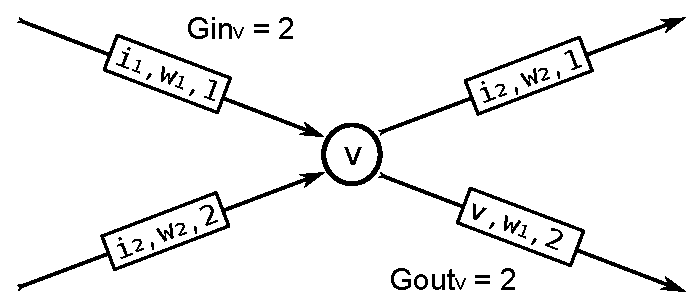
\includegraphics[bb=110 613 432 747,scale=0.7]{./figs/B_GL_Multi.eps}
	% B_GL_Multi.eps: 0x0 pixel, 300dpi, 0.00x0.00 cm, bb=110 613 432 747
	\caption{Exemplo com Grau L�gico de Entrada e Sa�da iguais.}
	\label{fig:B_GL}
\end{figure}

Na Figura \ref{fig:B_GL} est� um exemplo onde o n� $v$ tem grau l�gico de entrada e sa�da iguais a $2$. Dentre os componentes que partem de $v$, um deles
comp�e uma liga��o l�gica iniciada em $i_2$, que n�o est� representado na figura, bem como o destino desta liga��o, que passa transparetemente por $v$.
Apenas um componente com valor $2$ inicia liga��es l�gicas em $v$, por isso $GLout_v = 2$. Por sua vez, $2$ componentes incidem em $v$ trasportando
liga��es l�gicas iniciadas em $i_1$ e $i_2$, cuja soma � $3$, mas como uma passa transparetemente vindo de $i_2$, ent�o $GLin_v = 2$. Os componentes que
incidem em $v$ pertecem a dois planos l�gicos ($w_1$ e $w_2$), assim como os que nele se iniciam. Mas $v$ possui duas liga��es l�gicas de entrada em planos
distintos, e as de sa�da todas no plano $w_1$. Ainda nesta figura, a multiplicidade de liga��es l�gicas  ($Ml$) entre o par $(i_1,v)$ � $1$, e entre o par
$(i_2,v)$ tamb�m. Consequentemente, a multiplicidade por plano desses pares ($PMl$) tamb�m � $1$

\section{Minimiza��o do Congestionamento}
\label{Cong}

O caso de uso apresentado nesta se��o, mostra que � poss�vel minimizar diretamente o congestionamento nesta modelagem, pois 
esta � uma bem conhecida m�trica para o VTD. Todavia, uma abordagem mais eficiente � a simples limita��o do congestionamento, 
minimizando outra m�trica, de modo a deixar o modelo mais trat�vel \cite{Renato06}, como foi usado na forma b�sica do modelo 
TWA.

\subsection{Mantendo a Multiplicidade de Liga��es L�gicas}

Como foi comentado na Se��o \ref{Basic}, a multiplicidade das liga��es l�gicas fica impl�cita nas vari�veis de 
distribui��o de tr�fego ($q_{sw}^{ij}$). Deste modo, n�o � poss�vel minimizar diretamente o tr�fego em cada liga��o l�gica, o congestionamento. Para
minimiz�-lo mantendo esta multiplicidade, s�o necess�rias novas vari�veis para contabilizar o tr�fego em cada canal. 
Para enumerar as liga��es l�gicas
entre um par $(i,j)$ s�o definidos a seguir o �ndice $r$ e as vari�veis de fra��o de tr�fego $f_{ij}^r$ e liga��o l�gica $F_{ij}^r$.

\begin{notation}
O �ndice $r\in\{1,\cdots,CapLog_{ij}\}$ enumera os poss�veis m�ltiplos canais l�gicos entre par $(i,j)$, onde $CapLog_{ij}$ 
� o menor valor entre $GLout_i$ e $GLin_j$. 
\label{indice:r}
\end{notation}

% \zz
\begin{var}
Fra��o de Tr�fego $=$ $f_{ij}^r \in [0,1]$: vari�vel cont�nua.
 \label{f}
\end{var}

% \zz
\begin{var}
Liga��o L�gica $=$ $F_{ij}^r \in \{0,1\}$: vari�vel bin�ria.
 \label{F}
\end{var}

% \zz
\begin{var}
 \label{FmaxVar}
$F_{max}$ $=$ Fra��o de tr�fego do canal mais carregado da rede (congestionamento).
\end{var}

A aqui optou-se por limitar o �ndice $r$ em fun��o do grau l�gico, pois este � um controle comum nos trabalhos que tratam do congestionamento
\cite{Sivarajan01, ram02}. Consequentemente, para controlar o grau
l�gico, tamb�m ser�o necess�rias as Restri��es \ref{cases:rest:GLin} e \ref{cases:rest:GLout} da se��o anterior. O congestionamento � definido na vari�vel
$F_{max}$ (Vari�vel \ref{FmaxVar}). Supondo que $GLout_v = GLin_v = GL$ para todo $v$, ou seja, a rede possui grau l�gico uniforme, o n�mero de vari�veis
bin�rias adicionadas ao modelo seria $N^2\cdot GL$, idem para vari�veis cont�nuas. Supondo ainda que $GL < N$, o que � bem razo�vel, n�o haveria autera��o
no n�mero de vari�veis do modelo b�sico, assimtoticamente.

Todavia, no lugar do grau l�gico, outro controle poderia ser usado se for conveniente, como a multiplicidade de
liga��es l�gicas ($Ml$), definida na se��o anterior. Mas deve-se tomar cuidado nessa escolha, pois o controle usado influencia diretamente na quantidade e
vari�veis que ser�o adicionadas ao modelo, podendo ultrapasar a ordem de grandeza do n�mero de vari�veis na forma b�sica do TWA.

A seguir est�o relacionadas as restri��es necess�rias para o controle do congestionamento, que feito pela Fun��o Objetivo abaixo:

\textbf{Fun��o Objetivo}

\begin{itemize}

\item Minimizar o Congestionamento

\begin{equation} 
     F_{max}
\label{cases:fo:Hmax}
\end{equation}

\end{itemize}

\textbf{Restri��es}

\begin{itemize}
	\item Liga��es L�gicas

\begin{equation}
 \sum_{wm} B_{iw}^{mv} - \sum_{wn} B_{iw}^{vn} = \sum_r F_{iv}^r\Forall{(i,v)} \text{, com } i\neq v.
\label{cases:rest:Hmax_Log}
\end{equation}

	\item Controle do Tr�fego em cada Liga��o L�gica

\begin{equation}
F_{ij}^r \geqslant f_{ij}^r \Forall{(i,j,r)}.
\label{cases:rest:Hmax_Flow}
\end{equation}

\begin{equation}
\sum_{sw} q_{sw}^{ij}\cdot A_s = Cap\cdot \left(\sum_r f_{ij}^r \right) \Forall{(i,j)}.
\label{cases:rest:Hmax_Eq_Flow}
\end{equation}

	\item Congestionamento

\begin{equation}
F_{max} \geqslant f_{ij}^r\Forall{(i,j,r)}.
\label{cases:rest:Hmax}
\end{equation}

\end{itemize}

A Restri��o \ref{cases:rest:Hmax_Log} determina as liga��es l�gicas $F_{ij}^r$ em termos dos componentes topol�gicos. Semelhante � Restri��o
\ref{cases:rest:Ml} da se��o anterior, que limita a multiplicidade de liga��es l�gicas entre o pares $(i,v)$, a Restri��o \ref{cases:rest:Hmax_Log} iguala
esse valor � soma das vari�veis bin�rias $F_{ij}^r$ associadas a esse par. Deste modo haver� $F_{ij}^r \neq 0$ em quantidade igual a multiplicidade de
liga��es entre o par $(i,v)$. Assim, a Restri��o \ref{cases:rest:Hmax_Log} � equivalente � equa��o \ref{eq:DiffivLog}. A forma desta equa��o � uma maneira
conhecida de se associar numeros inteiros � vari�veis bin�rias \cite{cormen02}.

\begin{equation}
  \sum_{w}LL_{iv}^w = \sum_r F_{iv}^r \Forall{(i,v)},\, \mbox{\small$i\neq v$} 
   \label{eq:DiffivLog}
\end{equation}


A fra��o de tr�fego $f_{ij}^r$ (Vari�vel \ref{f}) � semelhante a Vari�vel \ref{FlowVar} (fra��o de fluxo - $q_{sw}^{ij}$), com a diferen�a 
de que a Vari�vel \ref{f} separa o fluxo por canal, e a outra considerava todos como um �nico caminho.
Para associar tr�fego �s liga��es l�gicas, a Restri��o \ref{cases:rest:Hmax_Flow} define a fra��o do tr�fego em cada liga��o, limitada pela
exist�ncia do canal. Se n�o n�o h� uma liga��o associada a um determinado �ndice $r$, n�o haver� tr�fego nessa liga��o.

A Restri��o \ref{cases:rest:Hmax_Eq_Flow}, em conjunto com a a restri��o de limita��o de capacidade do modelo b�sico do TWA
(Restri��o \ref{rest:DefCapFlow}), garante equival�ncia entre o tr�fego que � alocado nas vari�veis $q_{sw}^{ij}$ e o que distribu�do nas vari�veis
$f_{ij}^r$. A Restri��o \ref{rest:DefCapFlow} � repetida na equa��o \ref{eq:DefCapFlowBasic} para facilitar a compree��o desse relacionamento. As vari�veis
$q_{sw}^{ij}$ � quem de fato fazem o roteamento do tr�fego pela rede, levando as demandas de tr�fego da origem at� seu destino. As vari�veis $f_{ij}^r$
apenas separam o tr�fego nas m�ltiplas liga��es l�gicas entre o par $(i,j)$, sem informa��o sobre origem ou destino. Essa fun��o n�o � exercida pelas
vari�veis $q_{sw}^{ij}$, mas � indispens�vel para o controle do congestionamento. A Restri��o \ref{cases:rest:Hmax_Eq_Flow} apenas garante que todo o
tr�fego roteado pela rede foi distribu�do nas liga��es l�gicas independentemente, e vice-ver�a.

Como a vari�vel $f_{ij}^r$ � limitada pela exist�ncia da liga��o l�gica $F_{iv}^r$ na Restri��o \ref{cases:rest:Hmax_Flow}, o tr�fego separado nas liga��es
l�gicas entre o par $(i,v)$ tamb�m � limitado pela multiplicidade de liga��es entre esse par. Isso � mostrado na equa��o \ref{eq:DiffivLogM}. Portanto,
esse tr�fego tamb�m � limitado pela capacidade combinada dessas liga��es, como mostra a equa��o \ref{eq:DiffivLogCap}, cujo lado direito da desigualdade �
igual ao da Restri��o de limita��o de capacidade do modelo b�sico do TWA (Restri��o \ref{rest:DefCapFlow}).

\begin{equation}
\sum_{s} q_{sw}^{iv}\cdot A_s \leqslant Cap\cdot \left(\sum_{m} B_{iw}^{mv} - \sum_{n} B_{iw}^{vn}\right) \Forall{(i,v,w)} \mbox{, com $i\neq v$}
\label{eq:DefCapFlowBasic}
\end{equation} 
 
\begin{equation}
  \sum_{w}LL_{iv}^w \geqslant \sum_r f_{iv}^r \Forall{(i,v)},\, \mbox{\small$i\neq v$} 
   \label{eq:DiffivLogM}
\end{equation}
 
\begin{equation}
Cap\cdot \left(\sum_r f_{ij}^r \right) \leqslant Cap\cdot \left(\sum_{w}LL_{iv}^w \right) \Forall{(i,v)},\, \mbox{\small$i\neq v$} 
   \label{eq:DiffivLogCap}
\end{equation}

Por fim, o congestionamento ($F_{max}$) � definido na Restri��o \ref{cases:rest:Hmax} em termos das fra��es de tr�fego $F_{iv}^r$,
como o tr�fego na liga��o l�gica mais carregada. Deste modo, a Fun��o Objetivo \ref{cases:fo:Hmax} agora consiste em minimizar $F_{max}$, substituindo a
fun��o objetivo do modelo b�sico. 

\subsection{Sem Multiplicidade de Liga��es L�gicas}

Uma forma alternativa, e bem mais simples, para se minimizar diretamente o congestionamento � adotando a Restri��o
\ref{cases:rest:Ml}, de controle da multiplicidade de liga��es, com $Ml=1$. Todavia, perde-se assim a capacidade de se obter
solu��es com liga��es l�gicas m�ltiplas. 
Mas, a vantagem � que pode-se minimizar o congestionamento adotando apenas a Restri��o \ref{Hmax} a seguir, al�m da Vari�vel \ref{FmaxVar} e a Fun��o
Objetivo
\ref{cases:fo:Hmax}, definidas acima.

A Restri��o \ref{Hmax} define o congestionamento da mesma forma que a restri��o \ref{cases:rest:Hmax} o fez acima. Mas desta vez isto � feito diretamente
sobre as fra��es de fluxo $q_{sw}^{ij}$, somando todo o tr�fego passando pela liga��o l�gica $(i,j)$, onde agora n�o h� multiplicidade. Deste modo, o
tr�fego em cada $(i,j)$ estar� apenas em um plano l�gico.

\textbf{Restri��o}

\begin{itemize}

 \item Congestionamento:

\begin{equation}
F_{max} \geqslant \sum_{sw} q_{sw}^{ij}\cdot A_s \Forall{(i,j)} \text{, com } Ml=1
\label{Hmax} 
\end{equation}

\end{itemize}

\subsection{Sem Multiplicidade de Liga��es L�gicas em cada Plano L�gico}

Uma terceira forma para se poder controlar diretamente o congestionamento � adotando a Restri��o
\ref{cases:rest:PMl}, de controle da multiplicidade de liga��es por plano l�gico, com $PMl=1$. Deste modo perde-se apenas a multiplicidade de liga��es em
cada plano, mas ainda pode haver $W$ liga��es m�ltiplas para cada par $(i,j)$. Assim, pode-se minimizar o congestionamento adotando apenas a Restri��o
\ref{HmaxW} a seguir, al�m da Vari�vel \ref{FmaxVar} e a Fun��o
Objetivo
\ref{cases:fo:Hmax}, definidas acima. 

\textbf{Restri��o}

\begin{itemize}

 \item Congestionamento:

\begin{equation}
F_{max} \geqslant \sum_{s} q_{sw}^{ij}\cdot A_s \Forall{(i,j,w)} \text{, com } PMl=1
\label{HmaxW} 
\end{equation}

\end{itemize}

A Restri��o \ref{HmaxW} define o congestionamento da mesma forma que a restri��o \ref{Hmax} o fez. Mas desta vez, o tr�fego � separado por comprimento de
onda, como na Restri��o \ref{rest:DefCapFlow} de limita��o de capacidade no modelo b�sico. Deste modo, o tr�fego em cada $(i,j)$ poder� estar em
todos os planos l�gicos, mas sem multiplicidade em cada um.

\section{Liga��es L�gicas em cada Fibra}
\label{LimW}

Um controle muito usado nas modelagens de RWA  \cite{Zang00,Jaumard04}, � o n�mero m�ximo de 
liga��es l�gicas por liga��o f�sica ($L$), Vari�vel \ref{LimWd}. Ele limita a densidade da multiplexa��o de
comprimentos de onda por liga��o f�sica, um importante aspecto de Redes �pticas WDM \cite{ramamurthy99}. 

A vari�vel $L$ pode ser minimizada diretamente na
Fun��o Objetivo \ref{cases:fo:L} ou, caso seja fixada, ela pode ser usada como limite superior em cada liga��o f�sica, como � feito na Restri��o \ref{L}.
Esta restri��o limita  indiretamente a capacidade dos n�s realizarem liga��es l�gicas. Pois, dentre as liga��es l�gicas que passam por uma liga��o f�sica
de entrada, por exemplo, uma parte ir� passar transparetemente. Ent�o, a quantidade deliga��es l�gicas incidentes por esta fibra tamb�m est� limitada por
$L$. Analogamente, isso se estende para todas as liga��es f�sicas de entrada e sa�da.


% \zz
\begin{var}
 \label{LimWd}
$L$ $=$ N�mero m�ximo de liga��es l�gicas em cada liga��o f�sica.
\end{var}

\textbf{Fun��o Objetivo}

\begin{itemize}

\item Minimizar o M�ximo de Liga��es L�gicas em Cada Liga��o F�sica

\begin{equation} 
     L
\label{cases:fo:L}
\end{equation}

\end{itemize}

\textbf{Restri��o}

\begin{itemize}

 \item Liga��es L�gicas em Cada Liga��o F�sica:

\begin{equation}
 \label{L}
\sum_{iw} B_{iw}^{mn}\leqslant L\Forall{(m,n)}.
\end{equation}

\end{itemize}


\section{N�mero de Saltos F�sicos}

Uma m�trica importante para o projeto de redes �pticas � o n�mero de saltos f�sicos da topologia \cite{Zang00}. Este valor 
� minimizado na Fun��o Objetivo \ref{cases:fo:B}, atrav�s da soma de todos os componentes topol�gicos, pois cada componente 
topol�gico representa um salto f�sico. Uma propriedade importante desta abordagem � que ela evita o aparecimento de 
ciclos na topologia. O ideal seria minimizar a dist�ncia percorrida por cada enlace l�gico, o que promoveria um controle mais eficiente da degrada��o do
sinal �ptico.
Minimizar o n�mero total de saltos pode ser adotado por uma quest�o de compatibilidade com outros modelos, como os resultados encontrados em
\cite{Karcius04}, que
ser�o usados na compara��o dos experimentos computacionais do Cap�tulo \ref{cap:testes-sec:karcius}.

\textbf{Fun��o Objetivo}

\begin{itemize}

\item Minimizar o M�ximo de Liga��es L�gicas em Cada Liga��o F�sica

\begin{equation} 
     \sum_{imnw} B_{iw}^{mn}
\label{cases:fo:B}
\end{equation}

\end{itemize}

% % % As vari�veis de fra��o de fluxo agregado, definidas no modelo b�sico, s�o suficientes para modelar a distribui��o do tr�fego, embora na implementa��o
% real % de
% % % m�ltiplas rotas f�sicas entre um mesmo par de n�s $(i,j)$, alguns detalhes ainda carecem ser decididos, pois podem haver mais de uma maneira de
% % configura-los. Um
% % % exemplo disso � dado na Figura \ref{fig:Unsolved}, onde o conjunto de componentes topol�gicos dado permite duas possibilidades de 
% % % configura��o dos percursos l�gicos. � garantida implicitamente a aloca��o de recursos suficientes, mas este sub-problema fica sem ser resolvido pelo
% % modelo. 
% % % Por essa raz�o, n�o � poss�vel controlar a real dist�ncia percorrida pelas demandas de tr�fego, sendo este um preju�zo da
% % % modelagem TWA.
% % % 
% % % Essas situa��es podem ser tratadas considerando outros fatores, como a dist�ncia entre os 
% % % n�s. Mas s�o quest�es de menor complexidade, se a topologia j� estiver decidida, e podem ser resolvidas na fase 
% % % de configura��o da rede. Isso n�o influencia na modelagem dos recursos da rede e portanto n�o ser� tratado aqui.
% % % 
% % % \begin{figure}[htb]
% % %  \centering
% % %  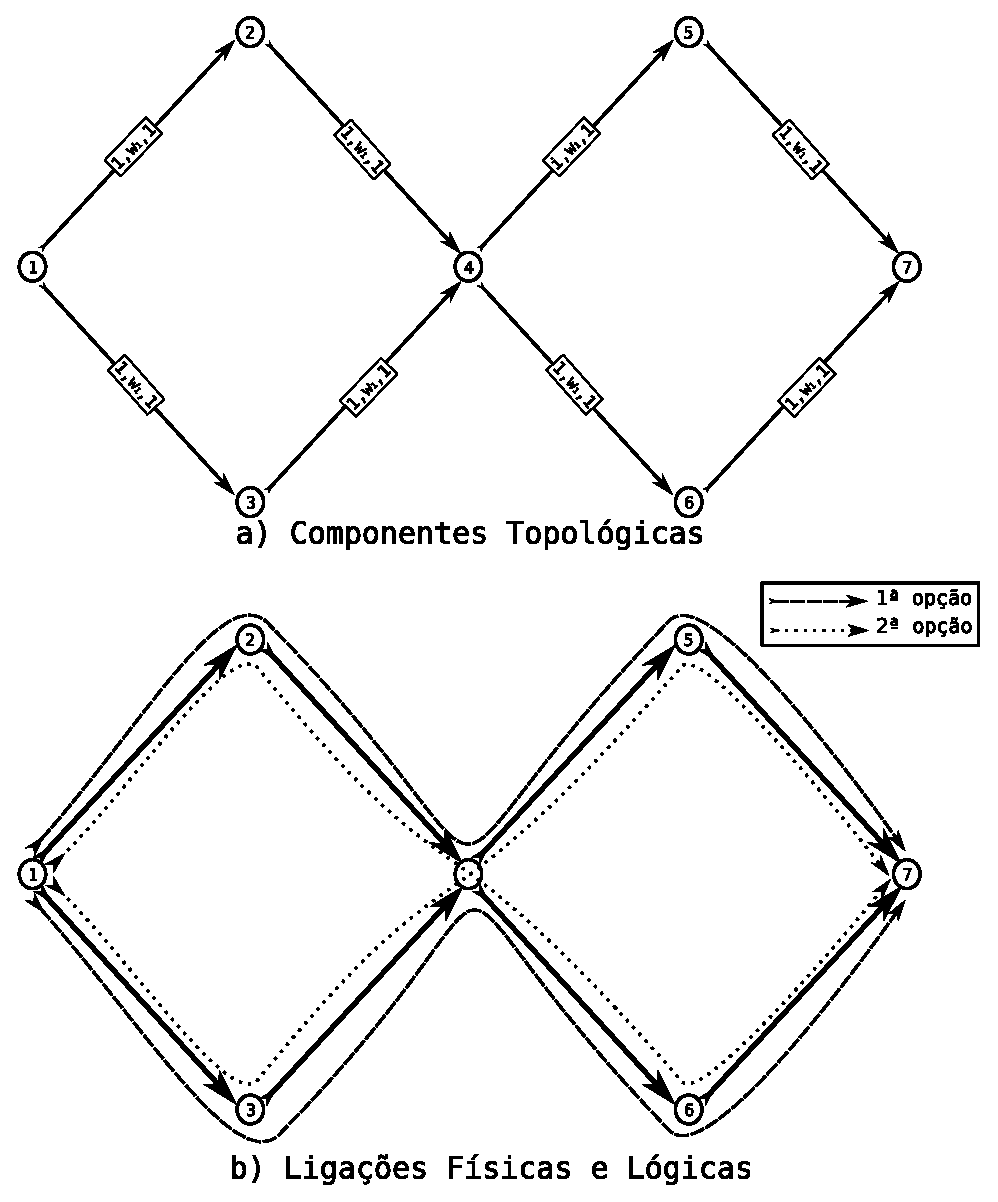
\includegraphics[bb=71 267 541 759, scale=0.8]{figs/unsolved.eps}
% % %  % unsolved.eps: 1179666x1179666 pixel, 300dpi, 9987.84x9987.84 cm, bb=70 210 533 771
% % %  \caption{Em $b)$ vemos duas poss�veis de interpreta��es dos componentes topol�gicos em $a)$.}
% % %  \label{fig:Unsolved}
% % % \end{figure}


\section{Minimiza��o do N�mero de Comprimentos de Onda}
\label{CtrlW}

Um objetivo comum nas modelagens do RWA � minimizar o n�mero de comprimentos de onda utilizados na rede \cite{Zang00, 
Jaumard04}. Esse n�mero, na forma b�sica do TWA, � um dos dados que definem uma inst�ncia do modelo, deixando uma quantidade $W$ de comprimentos de onda
dispon�veis para serem usados. Nesta se��o � introduzida a possibilidade de minimizar diretamente a quantidade que ser� utilizada. A seguir est�o as
defini��es necess�rias. Mais uma vez, isso � feito para oferecer compatibilidade com outras modelagens da literatura \cite{Zang00}. Todavia, uma abordagem
diferente foi utilizada para o mesmo objetivo
nos experimentos computacionais do Cap�tulo \ref{cap:testes}.

\begin{var}
 \label{Cw}
Seja $Q_w\in\{0,1\}$, com $w \in \{1,..,W\}$. $Q_w = 1$ se o comprimento de onda $w$ � utilizado na rede e $Q_w = 0$ caso contr�rio.
\end{var}

\textbf{Fun��o Objetivo}

\begin{itemize}

\item Minimizar o N�mero de Comprimentos de Onda:

\begin{equation} 
     \sum_w Q_w
\label{cases:fo:W}
\end{equation}

\end{itemize}

\textbf{Restri��o}

\begin{itemize}

 \item N�mero de Comprimentos de Onda:

\begin{equation}
 \label{cases:rest:Qw} 
\sum_{vn} B_{vw}^{vn} \leqslant K\cdot (N^2 - N)\cdot Q_w \Forall{w}.
\end{equation}

\end{itemize}

Se em um plano l�gico $w$ h� uma rota f�sica ou mais. Cada uma destas � facilmente associada ao primeiro componente
em seu percurso, dada a agrega��o utilizada no roteamento dos comprimentos de onda. Uma liga��o l�gica neste plano, iniciada em $v$, est�
associada a um componente da forma $B_{vw}^{vn}$, para algum $n$. Ou seja, se algum desses componentes for n�o nulo, ent�o o comprimento de onda $w$ foi
utilizado. Isso pode ser determinado pela soma desses componentes, como est� expresso na equa��o \ref{eq:QwEQ}. 

\begin{equation}
	\sum_{vn} B_{vw}^{vn} \neq 0 \Longleftrightarrow Q_w = 1
	\label{eq:QwEQ}
\end{equation}

Para descrever essa situa��o na forma de uma
restri��o linear, � necess�rio apenas garantir que $Q_w = 1$ quando $w$ for utilizado. Pois, como $Q_w$ ser� minimizado, casos em que $Q_w = 1$, sem nada
que o exija na modelagem, ser�o evitados pela fun��o objetivo. Assim, � necess�rio modelar apenas a equa��o \ref{eq:QwVolta}. Isso � feito com uma
equa��o da forma \ref{eq:Qw}, onde $H$ pode ser qualquer fator positivo, que seja sempre maior ou igual ao somat�rio � esquerda da desigualdade. Um valor
mais adequado para o fator $H$ � o n�mero m�ximo que o somat�rio pode assumir. Esse valor � $K\cdot (N^2 - N)$, pois existem $N^2 - N$ combina��es
poss�veis para o par $(v,n)$, e cada uma pode estar associada � $K$ liga��es f�sicas paralelas. Em fim, substituindo $H$ na equa��o \ref{eq:Qw} chagamos �
Restri��o \ref{cases:rest:Qw}.

\begin{equation}
	\sum_{vn} B_{vw}^{vn} \neq 0 \Longrightarrow Q_w = 1
	\label{eq:QwVolta}
\end{equation}

\begin{equation}
 \label{eq:Qw} 
\sum_{vn} B_{vw}^{vn} \leqslant H\cdot Q_w \Forall{w}.
\end{equation}

\subsection{Topologia F�sica Fixa}

Se a topologia f�sica seja � pr�-definida como dado do problema, diz-se que a topologia f�sica � fixa. Neste caso, h� uma forma alternativa para se modelar
$Q_w$, que reaproveita uma das restri��es do modelo TWA. Assim, evita-se acrescentar a Restri��o \ref{cases:rest:Qw} ao modelo, dixando-o mais conciso. Se a
vari�vel de topologia f�sica $D_{mn}$ (Se��o \ref{cap:twa-sec:VarFis}) for fixada, podemos multiplic�-la por $Q_w$ na Restri��o \ref{rest:DefFis} do modelo
b�sico, sem prejudicar a fun��o original da restri��o, e obter o mesmo efeito da Restri��o \ref{cases:rest:Qw}. Com a diferen�a que agora est� separada por
par $(m,n)$ e o fator $H$ foi substituido por $D_{mn}$. Deste modo, se a toplogia f�sica em um dado de entrada, a Restri��o \ref{cases:rest:FisQw} deve
substituir a equa��o \ref{rest:DefFis} do modelo original, e a Restri��o \ref{cases:rest:Qw} n�o ser� necess�ria.

Para minimizar diretamente o n�mero de comprimentos de onda utilizados na rede, basta usar a soma de todas as 
vari�veis $Q_w$ (Vari�vel \ref{Cw}) na Fun��o Objetivo \ref{cases:fo:W}.

\textbf{Restri��o}

\begin{itemize}

 \item N�mero de Comprimentos de Onda:

\begin{equation}
\sum_i B_{iw}^{mn} \leqslant Q_w\cdot D_{mn}\Forall{(m,n,w)}.
\label{cases:rest:FisQw}
\end{equation} 

\end{itemize}


\section{Convers�o entre Comprimentos de Onda}
\label{Conv}

Outro cen�rio comum nas modelagens para o RWA � a possibilidade de convers�o do comprimento de onda ao longo de um caminho �ptico. H� 
duas formas mais comuns de se tratar essa abordagem: ou um n� possui capacidade total de convers�o \cite{Zang00, Jaumard04, Tornatore07} e todas 
as liga��es l�gicas passando por ele podem mudar de comprimento de onda; ou h� uma quantidade m�xima de convers�es \cite{ram98, 
Karcius04}. O primeiro m�todo � apenas um caso particular do segundo, deste modo, trataremos do caso mais geral.

Inicialmente, ser� condiderado um caso particular, quando o topologia f�sica da rede �m um dos dados de entrada do problema. Neste caso, diz-se que a
topologia f�sica � fixa. Em seguida, ser� tratado o caso geral, com a topologia f�sica como uma das vari�veis do problema. 

Como o projeto aqui modelado pretende servir de base para o dimensionamento da rede, n�o ser� fixado quais n�s ter�o a capacidade de convers�o, mas sim
controlaremos o n�mero de convers�es na rede pela Vari�vel \ref{x}. 

\begin{figure}[htb]
	\centering
	\includegraphics[bb=0 0 596 843,scale=0.7]{./figs/desvios.eps}
	% desvios.eps: 0x0 pixel, 300dpi, 0.00x0.00 cm, bb=0 0 596 843
	\caption{Possibilidades de desviar uma Rota}
	\label{fig:desvios}
\end{figure}

Ao se habilitar um n� a realizar convers�es de comprimento de onda, torna-se necess�rio utilizar uma restri��o mais geral, que garante a conserva��o fixada
a
origem, mas independente do comprimento de onda. A Restri��o \ref{ConservLogC} cumpre esse papel. Ela sozinha j� habilita o n� com capacidade de convers�o
total, onde todo comprimento de onde que chega pode ser convertido livremente. J� o n�mero de convers�es � considerado na Restri��o \ref{ConservLogCx}, que
substitui a Restri��o \ref{rest:DefCapFlow}.

\begin{var}
 \label{x}
Em um n� intermedi�rio $v$, o n�mero de rotas com com origem $i$ e comprimento de onda $w$ desvias � $x_{iv}^w \in \{0, \cdots, \sum_n
D_{vn}\}$, com topologia f�sica fixa. 
\end{var}

\textbf{Fun��o Objetivo}

\begin{itemize}
\item Minimizar o N�mero de Convers�es:
\begin{equation}
 \label{ObjX}
\sum_{imw} x_{im}^w
\end{equation}
\end{itemize}

\textbf{Restri��es}
\begin{itemize}
\item Conserva��o de Rotas sem Continuidade de Comprimento de Onda:
\begin{equation}
 \label{ConservLogC}
 \sum_{nw} B_{iw}^{nm} \geq \sum_{nw} B_{iw}^{mn}\Forall{(i,m)} \text{, com } i\neq m.
\end{equation}

\item Continuidade de Comprimento de Onda com Taxa de Desvio:
\begin{equation}
 \label{ConservLogCx}
 \sum_{s} q_{sw}^{ij}\cdot A_s \leqslant Cap\cdot \left(\sum_{m} B_{iw}^{mj} - \sum_{n} B_{iw}^{jn} - x_{ij}^w\right) \Forall{(i,j,w)}
\end{equation}
\end{itemize}

Note na defini��o da Vari�vel \ref{x}, que o comprimento de onda de sa�da do conversor n�o � registrado. A Restri��o \ref{ConservLogCx} 
assegura que haver� componentes topol�gicos no comprimento de onda $w$, com origem $i$, chegando em $m$ em n�mero suficiente para realizar as 
convers�es. Para cada uma destas, a Restri��o \ref{ConservLogC} garante que haver� algum componente partindo de $m$, com origem $i$, mas em um 
comprimento de onda diferente de $w$. 

Aqui tamb�m podem ocorrer situa��es nas quais algo 
fica indefinido na interpreta��o dos componentes. Mas esses casos tamb�m n�o influenciam na modelagem e por isso tamb�m n�o ser�o aqui 
considerados. % como a que foi ilustrada na Figura \ref{fig:Unsolved}, 

Pode ser conveniente limitar o n�mero de convers�es em cada n�, ou seja, limitar a soma $\sum_{iw} x_{im}^w$, ou o n�mero total de convers�es. 
Ou ainda, usar este �ltimo como fun��o objetivo, o que � feito pela Restri��o \ref{ObjX}.


\subsection{Topologia F�sica Vari�vel}

Quando a topologia f�sica � uma das vari�veis do problema, � necess�rio definir um limite para o n�mero de liga��es f�sicas originadas em cada
n� da rede ($GFout_v$).

\begin{dados}
 $GFout_v$ $=$ N�mero m�ximo de liga��es f�sicas que podem originar-se no n� $v$.
\end{dados}

\begin{var}
 \label{xv}
Em um n� intermedi�rio $v$, o n�mero de rotas com com origem $i$ e comprimento de onda $w$ desvias � $x_{iv}^w \in \{0, \cdots, GFout_m\}$, com topologia
f�sica � livre. 
\end{var}

Se a topologia f�sica � conhecida, ou seja, sendo dados os valores para $D_{mn}$, ent�o $x_{im}^w$ j� est� bem definida, caso contr�rio, ser� necess�ria a
restri��o adicional \ref{Defx}.

\textbf{Restri��o}
\begin{itemize}
\item Limita��o de Convers�es:
\begin{equation}
 \label{Defx}
x_{iv}^w \leq \sum_n D_{vn}\Forall{(i,v,w)}.
\end{equation}
\end{itemize}




%%%%%%%%%%%%%%%%%%%%%%%%%%%%%%%%%%%%%
%% Lower Bounds
%% Copyright 2009 Fabio de Oliveira Lima.
%% Este documento � distribu�do nos termos da licen�a 
%% GNU General Public License v2.
%%%%%%%%%%%%%%%%%%%%%%%%%%%%%%%%%%%%%


\chapter{Limitantes Inferiores}
\label{lb}


Nos trabalhos encontrados na literatura, no que diz respeito ao congestionamento, encontrar boas solu��es � uma tarefa f�cil para
heur�sticas \cite{Sivarajan01,Nina05}. Todavia, o c�lculo de limitantes inferiores (\textit{lower bounds} - LB) que garantam essa qualidade tem elevado
custo computacional, sendo esta
a parte mais dif�cil dessa abordagem. Apresentamos na se��o a seguir uma nova t�cnica para a obten��o de \textit{lower bounds} para o congestionamento. Ela
� uma formula de c�lculo direto, que denominamos \textit{Minimum Traffic Bound} (MTB), fornecendo um LB de alta qualidade para o
congestionamento, com custo computacional muito pequeno, cuja efici�ncia contrasta com as op��es encontradas na literatura \cite{ram96}. 

\section{MTB - Limitante Inferior para o Congestionamento}

Para determinar um LB para o congestionamento, precisamos estimar qual � o m�nimo de tr�fego que pode ser designado a cada liga��o l�gica da rede. N�o h�
uma
resposta direta, mas podemos fazer uma estimativa olhando cada n� independentemente. 
Na melhor das hip�teses, todo o tr�fego que passa pelas liga��es l�gicas
iniciadas em um n� $v$ � composto exclusivamente por demandas de tr�fego tamb�m originadas neste mesmo n�. Analogamente, o tr�fego nas liga��es l�gicas
incidentes em $v$ seria
composto por demandas destinadas a ele. Esses s�o os menores valores poss�veis, considerando que todo o tr�fego da rede ser� devidamente enviado e recebido.

Assim,  dividindo todo o tr�fego originado em $v$ pelo n�mero de liga��es l�gicas nele iniciadas,
temos uma estimativa do menor tr�fego poss�vel nessas liga��es l�gicas. Analogamente, uma estimativa pode ser feita para o tr�fego destinado a $v$ nas
liga��es l�gicas nele incidentes. Extrapolando isso para toda a rede, a maior dentre essas estimativas seria uma boa
candidata a limitante inferior para o congestionamento. Isto porque n�o � poss�vel que um n� envie menos tr�fego do que a soma das demandas originadas
nele. E analogamente, n�o � poss�vel que um n� receba menos tr�fego do que o destinado a ele. O MTB � assim definido como o m�nimo dos valores calculados
nas equa��es do conjunto de Dados \ref{MT}. 

Para estabelecer o MTB, consideraremos apenas o n�mero de liga��es l�gicas iniciando ou terminando em cada n� da rede. Nas modelagens para o VTD, essa � toda a
informa��o dispon�vel sobre a topologia l�gica da rede. Mas em modelagens mais abrangentes, como o TWA, isso pode n�o
ser um dado de entrada.

% {\small
\begin{dados}
Sejam $\alpha_v$ o n�mero de liga��es l�gicas originadas em um n� $v$ e $\beta_v$ o n�mero de liga��es l�gicas incidentes em $v$.
Deste modo:
\begin{enumerate}
\item $\Theta_v = \displaystyle\sum_d P_{vd}/\alpha_v\quad$ 
\item $\Gamma_v = \displaystyle\sum_s P_{sv}/\beta_v$ 
% \item $\Omega_{v_1v_2} = \max\{\Theta_{v_1},\Gamma_{v_2}\}$
\item $MTB = \max_{v_1v_2} \{\Theta_v,\Gamma_v\}$
\end{enumerate}
\label{MT}
\end{dados}

As estimativas comentadas acima, para o tr�fego m�nimo saindo e chegando em cada liga��o l�gica incidente ou originada em $v$, s�o $\Theta_v$ e $\Gamma_v$,
respectivamente. 
% Segue que, $\Omega_{v_1v_2}$ � a estimativa de tr�fego m�nimo nas liga��es l�gicas entre o par $(v_1,v_2)$, que equivale ao maior valor
% entre as estimativas de tr�fego originado em $v_1$ ($\Theta_{v_1}$) e recebido em $v_2$ ($\Gamma_{v_2}$). 
Por sua vez, o MTB � definido como o m�ximo entre as
estimativas $\Theta_v$ e $\Gamma_v$. O teorema a seguir garante que o MTB � um LB para o congestionamento. Em sua demostra��o ser� necess�ria a proposi��o
abaixo.
% estimativas $\Omega_{v_1v_2}$. O teorema a seguir garante que o MTB � um LB para o congestionamento.

\begin{proposition}
   Para qualquer solu��o vi�vel de uma inst�ncia do VTD, para cada n� $v_1$ da rede ir� existir um n� $v_2$, tal que, h� uma liga��o l�gica entre o par
$(v_1,v_2)$ na solu��o, e o tr�fego nessa liga��o � maior ou igual � $\Theta_{v_1}$. Analogamente, haver� uma liga��o entre $(v_3,v_1)$, para algum n�
$v_3$, tal que, o tr�fego nessa liga��o � maior ou igual � $\Gamma_{v_1}$ 
\end{proposition}

\begin{proof}

Seja $\Phi_{v_1v_2}$ o tr�fego em uma liga��o l�gica $(v_1,v_2)$. � necess�rio demostrar que, em uma solu��o vi�vel qualquer:

\begin{equation}
(\forall\, v_1) \,(\exists\,v_2) \mbox{, tal que, }\Phi_{v_1v_2} \geqslant \Theta_{v_1}  
\label{lb:p1}
\end{equation} 

\begin{equation}
(\forall\, v_1) \,(\exists\,v_3) \mbox{, tal que, }\Phi_{v_3v_1} \geqslant \Gamma_{v_1}  
\label{lb:p2}
\end{equation} 

Ser� provado a seguir que a afirma��o em \ref{lb:p1} � verdadeira.

Seja $\Psi_{v}$ a soma de todo o tr�fego nas liga��es l�gicas iniciadas em $v$, em uma solu��o vi�vel qualquer. O m�nimo tr�fego que $v$ pode originar,
considerando todas as liga��es l�gicas iniciadas nele, � composto pelas demandas de tr�fego com origem em $v$, ou seja, $\sum_d P_{vd}$.  Considerando que
algum tr�fego possa ser retransmitido atrav�s de $v$, apos ser processado eletronicamente, conclui-se que:

\begin{equation}
\Psi_{v} \geqslant \sum_d P_{vd}
\label{lb:traf}
\end{equation} 

Seja $\overline{\Psi}_{v}$ o tr�fego m�dio das liga��es l�gicas iniciadas em $v$, em uma solu��o vi�vel qualquer. Dividindo os dois lados da inequa��o em
\ref{lb:traf} por $\alpha_{v}$, segue que: 

\begin{equation}
\frac{1}{\alpha_v}\cdot\left(\Psi_v \geqslant \sum_d P_{vd} \right) \quad \Longrightarrow  \quad
\frac{\Psi_v}{\alpha_v} \geqslant \frac{\sum_d P_{vd}}{\alpha_v} \quad \Longrightarrow \quad
\overline{\Psi}_v \geqslant \Theta_v
\label{lb:med}
\end{equation} 
% \overline{\Psi}_{v} = \frac{\Psi_{v}}{\alpha_{v}} \geqslant \frac{\sum_d P_{{v}d}}{\alpha_{v}} = \Theta_{v}

% Portanto, $\overline{\Psi}_v \geqslant \Theta_v$; o tr�fego m�dio saindo de $v$ � maior ou igual � $\Theta_{v}$.

Como foi provado em \ref{lb:med}, para todo n�
$v_1$, $\overline{\Psi}_{v_1}\geqslant \Theta_{v_1}$, em uma solu��o vi�vel qualquer. Assim, em alguma
liga��o l�gica iniciada em $v_1$, o tr�fego � maior ou igual � $\Theta_{v_1}$, ou seja, provou-se que \ref{lb:p1} � v�lida. A demostra��o para \ref{lb:p2} �
an�loga e ser� omitida.

\end{proof}


\begin{theorem}[\textit{Minimum Traffic Bound} -- MTB]
\label{MTB} 
Dado o n�mero de liga��es l�gicas originadas e incidentes em cada n� da rede, o MTB definido no conjunto de
Dados \ref{MT} � um limitante inferior para o congestionamento.
\end{theorem}

\begin{proof}
% Seja $(\zeta,\gamma)$ uma liga��o l�gica, parte de uma solu��o �tima para o VTD, cujo tr�fego corresponde ao valor �timo do congestionamento $\lambda_max*$.
% $$\Omega_{v_1v_2} \leqslant \lambda_{max}^* \Forall{(v_1,v_2)}$$  
% Para que isso seja v�lido, � suficiente que sejam verdadeiras as inequa��es a seguir:

Seja $\lambda_{max}^*$ o valor �timo do congestionamento. Para demostrar a validade do teorema, devemos demostrar que $MTB \leqslant \lambda_{max}^*$, o que
equivale a mostrar que sejam verdadeiras as inequa��es a seguir:

\begin{equation}
\Theta_{v} \leqslant \lambda_{max}^*\Forall{v}
\label{lb:i}
\end{equation} 

\begin{equation}
\Gamma_{v} \leqslant \lambda_{max}^*\Forall{v}
\label{lb:ii}
\end{equation} 

Para demostrar que a inequa��o \ref{lb:i} � v�lida, suponha por absurdo que ela � falsa, ou seja: 

\begin{equation}
\exists\,v \mbox{, tal que, } \Theta_v > \lambda_{max}^*
\label{lb:ni}
\end{equation} 

Do que foi suposto em \ref{lb:ni}, mais da conclus�o obtida em \ref{lb:p1}, se $\Theta_{v_1} > \lambda_{max}^*$, segue que $\Phi_{v_1v_2} > \lambda_{max}^*$
para qualquer solu��o vi�vel. O que � absurdo para as solu��es �timas, pois
contraria a defini��o de $\lambda_{max}^*$, como o tr�fego da liga��o l�gica mais carregada. Isso prova que a inequa��o \ref{lb:ni} � falsa, ou seja,
demonstra que \ref{lb:i} � verdadeira, como se queria. De modo an�logo pode-se verificar a validade da inequa��o \ref{lb:ii}, que conclui a
demostra��o do teorema.
%\bsq
% O que conclui a demostra��o. 
\end{proof}

Note que n�o foi feita restri��o quanto � multiplicidade de liga��es l�gicas, nem uniformidade do grau l�gico. Estamos considerando portanto o caso mais
geral do VTD. 

Dizemos que o MTB � um LB para para o VTD, pois a �nica restri��o feita � quanto ao conhecimento do n�mero de liga��es l�gicas iniciando e terminando em cada n�.
Em modelagens mais abrangentes, como o TWA, a introdu��o de mais restri��es e vari�veis pode fazer com que o �timo do VTD se torne invi�vel. Ainda assim, o MTB
ser� um LB para o congestionamento, todavia, outras t�cnicas de obten��o de LB poderiam ser empregadas para explorar o espa�o do conjunto de solu��es que se
tornou invi�vel. Uma alternativa � a conhecida t�cnica iterativa apresentada em \cite{ram02}.

O MTB foi aqui estabelecido em sua forma mais geral, considerando que cada n� pode possuir quantidades diferentes de liga��es l�gicas originadas ou incidentes,
entretanto, na literatura � comum considerar que os n�s da rede possuem grau l�gico uniforme \cite{ram02}. Neste caso, o MTB consiste no valor m�ximo do
do conjunto das somas das demandas originadas ou recebidas em cada n�, divido pelo grau l�gico da rede.
Portanto, conv�m apresentar uma formula��o mais direcionada para implementa��es. Isso � feito a seguir no Lema \ref{lem:MTB}.

\begin{lemma}
\label{lem:MTB}
 Se a rede possui grau l�gico uniforme $GL$, o MTB pode ser definido da seguinte forma:
 $$ \mbox{MTB} = \frac{1}{GL}\cdot\max_v \left\{\sum_d P_{vd},\sum_s P_{sv}\right\}$$
\end{lemma}


Em �ltima an�lise, o MTB explora a possibilidade da liga��o l�gica mais carregada da rede transportar predominantemente tr�fego que n�o foi ou n�o ser�
retransmitido. De fato, se $(i,j)$ � a liga��o mais carregada da rede, o ideal � que a maior parte de seu tr�fego seja destinado ao n� onde onde esta
liga��o l�gica incide ($j$). Pois do contr�rio, muito tr�fego seria retransmitido ao longo da rede, congestionando outras liga��es. Isso leva a crer que o
n� $j$ pode ter muito tr�fego a receber da rede. Por outro lado, quanto mais tr�fego for origin�rio de $i$, ouve menos retransmiss�o antes de chegar nele.

Tem-se ai duas tend�ncias que podem dominar a liga��o l�gica $(i,j)$: $j$ � o destino principal na rede, ou $i$ � o principal gerador de tr�fego. �
razo�vel que uma delas prevale�a. Por exemplo, se $j$ precisa receber mais tr�fego do que $i$ origina, seria melhor $i$ escoar esse tr�fego por
outra sa�da, que n�o $j$. Estendendo essa ideia a todo o projeto da topologia l�gica � de esperar que, na solu��o �tima, grandes emissores de tr�fego
tendem a n�o iniciar uma liga��o l�gica com destino a um grande receptor de tr�fego. E mesmo quando isso ocorresse, seria razo�vel que as duas tend�ncias
n�o concorressem numa mesma liga��o l�gica, mas sim, que a mais fraca tomasse caminhos alternativos. 

Deste modo, procurar por um LB se resumiria a encontrar a tend�ncia mais forte, seja de emiss�o ou recep��o. Essa � a ideia por tr�s do MTB, que apenas
investiga a matriz de demandas de tr�fego atr�s da maior tend�ncia. Esta suposi��o revelou-se v�lida empiricamente, posto que na maioria dos testes feitos o
MTB equivale ao �timo, como ser� visto no Cap�tulo \ref{cap:testes}. Por sorte, esse comportamento tem uma rela��o t�o direta com o grau l�gico de entrada e
sa�da dos n�s. 

Mas h� um ponto fraco nessa linha de pensamento. Ela depende que o tr�fego na liga��o l�gica mais carregada seja predominantemente caracterizado por sua
tend�ncia dominante. Isso tende a ser mais certo quanto mais assim�trica for matriz de demandas. Mas, se esta for fortemente uniforme, com pouca varia��o
entre o tamanho da demandas, a quantidade de tr�fego a ser retransmitida na rede superar� com facilidade as tend�ncias individuas de cada n�. Portanto, �
esperado que a qualidade do LB fornecido pelo MTB seja melhor em cen�rios de tr�fego assim�trico. Todavia, nos testes realizados no Cap�tulo
\ref{cap:testes}, mesmo para uma matriz com demandas uniformemente distribu�das, o MTB se mostrou bem eficiente.






% \subsection{Dichotomous Search Bound}
% 
% Uma forma de se obter \textit{lower bounds} para o congestionamento foi apresentada em \cite{ram02}. Esta t�cnica consiste
% na relaxa��o do modelo MILP, adicionando um \textit{lower} \textit{bound} conhecido $\lambda_{LB}$ � defini��o do congestionamento. O congestionamento
% $\lambda_{max}$ � a quantidade de tr�fego transportada pelo enlace l�gico mais solicitado $\lambda_{ij}$, ou seja, $\lambda_{max}\geq \lambda_{ij}$, $\forall
% i,j$. Se n�o h� um caminho l�gico entre os n�s $i$ e $j$ ($b_{ij}=0$), ent�o, $\lambda_{ij}=0$. Para obten��o de um novo LB para o congestionamento, �
% acrescentada a restri��o $\lambda_{max}\geq (1-b_{ij})\lambda_{LB}$, que pode ficar como $\lambda_{max}\geq \lambda_{ij}+(1-b_{ij})\lambda_{LB}$, sem modificar
% o
% modelo MILP. Todavia, relaxando a vari�vel bin�ria $b_{ij}$, permitindo que ela varie entre zero e um, esta defini��o para o $\lambda_{max}$ pode fornecer um
% valor superior a $\lambda_{LB}$, ou no m�nimo igual, mas, ainda sendo um LB para o congestionamento. 
% 
% Entretanto, �
% poss�vel usar uma ``previs�o' para se obter LBs, usando o m�todo iterativo. Pois, no modelo relaxado do ILB, n�o � necess�rio se conhecer um LB para poder
% produzir outro superior. Se, ao inv�s de entrarmos com um LB conhecido ($\lambda_{LB}$) na defini��o do congestionamento ($\lambda_{max}$), us�ssemos um valor
% qualquer $V$. Ter�amos a restri��o: 
% 
% \begin{equation}
% \label{hmaxv}
% \lambda_{max}\geq \lambda_{ij}+(1-b_{ij})V
% \end{equation} 
% 
% Para este contexto, faremos a seguir algumas defini��es. Sejam:
% 
% \begin{itemize}
%  \item $\lambda_{max}(V)$, os $\lambda_{max}$ definidos em fun��o deste $V$.
%  \item $W(V)=\min\{\lambda_{max}(V)\}$, o m�nimo dentre os $\lambda_{max}$ no modelo MILP relaxado, definidos pelo conjunto de restri��es na Equa��o \ref{hmaxv}
% acima. Ou seja, o �timo na relaxa��o do ILB, mas com $V$ no lugar de $\lambda_{LB}$.
% \item $Z^*$, o �timo do modelo MILP para uma dada inst�ncia.
% \end{itemize}
% 
% Segue que, se $V\geq Z^*$ ent�o $W(V)\leq V$, pois, no modelo MILP, setando este $V$, o �timo seria ele mesmo. Assim, na relaxa��o esta desigualdade �
% garantida.
% Pois, relaxando um modelo de minimiza��o, abrimos a possibilidade de encontrar uma solu��o menor. Mas, um modo equivalente de se escrever esta desigualdade �:
% se
% $W(V) > V$ ent�o $V<Z^*$. Ou seja, entrando com um valor qualquer no lugar do LB, no processo iterativo, se o resultado for maior que o valor passado, ent�o ele
% era de fato um LB para aquela inst�ncia. 






%%%%%%%%%%%%%%%%%%%%%%%%%%%%%%%%%%%%%
%% Experimentos Computacionais
%% Copyright 2009 Fabio de Oliveira Lima.
%% Este documento � distribu�do nos termos da licen�a 
%% GNU General Public License v2.
%%%%%%%%%%%%%%%%%%%%%%%%%%%%%%%%%%%%%


\chapter{Experimentos Computacionais com o TWA}
\label{cap:testes}

Para avaliar a pertin�ncia desta nova abordagem, testes computacionais foram realizados. Toda a modelagem do TWA foi descrita em AMPL�
(\textit{A Modeling Language for Mathematical Programming} - www.ampl.com), de modo que facilmente 
possa ser adaptada para v�rias finalidades. Utilizamos o \textit{solver} SCIP (\textit{Solving Constraint Integer Programs} - scip.zib.de) para resolver o modelo
MILP do TWA. Para interpretar o c�digo AMPL, gerando a entrada de dados para o SCIP, foi usado o GLPK (\textit{GNU Linear Programming Kit} -
www.gnu.org/software/glpk/). Vale observar que o SCIP e o GLPK s�o \textit{softwares} livres, de c�digo fonte aberto e de distribui��o gratuita.

Os resultados dos experimentos computacionais realizados com o TWA s�o comparados, neste cap�tulo, com os
publicados em \cite{Karcius04} e \cite{Sivarajan01}, aonde foram propostos modelos para a resolu��o integrada do VTD e RWA. 

A modelagem encontrada em \cite{Karcius04} � baseada nas modelagens cl�ssicas desses problemas \cite{ram02, Zang00}, o qual denominaremos \textbf{VTD-RWA}. Este
trabalho prop�e um algoritmo iterativo, que faz uso de programa��o linear, para resolver os problemas VTD e RWA de forma integrada. A solu��o do VTD gera
requisi��es para um conjunto de caminhos, representados pela topologia virtual, que devem ser roteados pela topologia f�sica. Os caminhos s�o alocados de maneira
a minimizar crit�rios de otimiza��o. A estrat�gia foi testada para redes com caracter�sticas distintas, mas n�o sendo considerado convers�o de comprimentos de
onda.

Para os resultados publicados em \cite{Sivarajan01}, � feita uma modelagem MILP que minimiza congestionamento em redes sem conversores de comprimentos de onda, o
qual denominaremos \textbf{KS}. Segundo os autores, esta formula��o n�o � computacionalmente trat�vel, sendo m�todos heur�sticos propostos. O Modelo MILP �
relaxado e executado interativamente por $25$ vezes usando um plano de corte. As vari�veis que representam a topologia virtual e os percursos f�sicos s�o
arredondadas, enquanto uma heur�stica de aloca��o de comprimentos de onda � aplicada para atribuir comprimentos de onda individualmente aos caminhos �pticos. O
tr�fego � roteado pela topologia virtual utilizando uma formula��o linear (LP) consistindo somente das restri��es de tr�fego do MILP relaxado. Uma das
desvantagens desse m�todo � que supondo que existam $W$ comprimentos de onda dispon�veis em cada fibra, o MILP relaxado obtem uma solu��o que satisfaz esta
restri��o. No entanto, sendo que o algoritmo de aloca��o de comprimentos de onda, que � aplicado subsequentemente, obtem solu��es sub�timas, n�o h� garantia de
uma aloca��o de comprimentos de onda com sucesso, respeitando o limite de $W$ comprimentos de onda. Como resultado, o m�todo n�o retorna necessariamente solu��es
vi�veis para todos os casos. 


\section{Compara��o com o modelo VTD-RWA}
\label{cap:testes-sec:karcius}

Nos resultados que iremos confrontar, s�o considerados: o grau l�gico da rede ($Gl$), o n�mero de liga��es l�gicas em cada fibra ($L$), o n�mero de comprimentos
de onda dispon�veis em cada liga��o f�sica ($W$) e o n�mero de saltos f�sicos na topologia ($S$). Esses par�metros s�o comumente tratados nas investiga��es a
cerca do RWA \cite{Zang00}.

Tamb�m � controlado o congestionamento, que � uma conhecida m�trica para o VTD. Isso � feito atrav�s da cl�ssica heur�stica HLDA \cite{ram02,
sbpo04}, gerando uma solu��o para o VTD que alimenta as etapas seguintes do procedimento, conforme apresentado em \cite{Karcius04}. Para cada grau
l�gico, o HLDA produz de forma determin�stica uma topologia l�gica, baseado na matriz de demandas. A solu��o para o VTD � completada distribuindo o
tr�fego sobre esta topologia, atrav�s de um modelo de programa��o linear \cite{ram02}.

Para produzir resultados pass�veis de compara��o, s�o acrescentadas � modelagem b�sica do TWA, mostrada na Se��o \ref{Basic}, as restri��es de 
controle do grau l�gico (Restri��o \ref{ConservGl}) e a de limita��o do n�mero de liga��es l�gicas em cada fibra (Restri��o \ref{L}). Esta formula��o 
espec�fica � denominada de TWA-$a$. Para controlar a qualidade das solu��es quanto ao congestionamento, foram obtidas topologias virtuais com uma 
implementa��o da heur�stica HLDA. Para cada uma destas topologias, foi distribu�do o tr�fego e calculado o congestionamento atrav�s do 
\textit{solver} do \textit{software} GLPK (\textit{GNU Linear Programming Kit} - www.gnu.org/software/glpk/), utilizando uma vers�o do 
modelo cl�ssico para o VTD \cite{ram02}. O valor de congestionamento obtido, arredondado para cima, foi usado como a capacidade dos canais 
l�gicos, na Restri��o (\ref{DefCapFlow}). Para cada inst�ncia, esse procedimento levou menos de um segundo, portanto n�o ser� 
considerado na contagem de tempo de processamento dos nossos resultados.

A estrat�gia adotada foi, partindo do menor grau l�gico ($Gl=1$), fixar nos valores m�nimos o n�mero de comprimentos de onda e a limita��o de 
liga��es das fibras ($W=1$ e $L=1$), minimizando o n�mero de saltos ($S$). Um solver para problemas MILP � instanciado com essa configura��o. 
Enquanto o solver retornar que o problema � insol�vel \cite{mukherjee}, $L$ ser� incrementado at� o seu limite, que � o valor atual de $W$. Quando 
$L$ n�o puder ser aumentado ($L=W$), ent�o $W$ o ser�, e assim por diante. Se uma solu��o vi�vel � encontrada, o solver � interrompido, a solu��o
� registrada e o grau l�gico � incrementado, dando continuidade ao processo.

% Se o solver n�o encontrar uma solu��o vi�vel dentro de $400$ segundos, ent�o ele � abortado e � aplicado o mesmo precedimento de quando a
% solu��o 
% � insol�vel. Isso � feito com o objetivo de ``afrouxar'' as restri��es de modo que o solver possa encontrar uma solu��o vi�vel mais rapidamente, 
% sacrificando um pouco a qualidade das restri��es. Se uma solu��o vi�vel � encontrada, dentro da janela de $400$ segundos, o solver �
% interrompido, 
% a solu��o � registrada e o grau l�gico � incrementado, dando continuidade ao processo. 

Nas situa��es em que o problema era insol�vel, o solver determinou isso em menos de um segundo, dificultando a separa��o dos tempos de leitura e
de execu��o. Portanto estes tempos n�o foram computados. Essas situa��es em que o modelo precisou ser calibrado, que chamaremos de
\textit{Inst�ncia Insol�vel} ($I$), fazem parte do m�todo e s�o registradas conjuntamente com os resultados.

% Este arranjo n�o foi obtido ao acaso e nem por tentativa e erro. O grau l�gico ($Gl$), o n�mero de comprimentos de onda ($W$), a limita��o de 
% liga��es l�gicas das fibras ($L$), a capacidade do canal ($Cap$) e o n�mero de saltos ($S$), deveriam ser controlados para viabilizar a compara��o 
% com o trabalho do Karcius. O par�metro $S$ foi escolhido para a fun��o objetivo pois, dentre as op��es, era a que fornecia o modelo mais enxuto. 
% Al�m disso, a minimiza��o do n�mero de saltos ajuda a evitar a forma��o de ciclos na solu��o \cite{Karcius04}. 

Como, nesta modelagem, $W$ est� diretamente relacionado a quantidade de vari�veis, � mais conveniente come�ar com $W=1$. Disso decorre a escolha 
de tamb�m come�armos com $Gl=1$ e $L=1$. A maior prioridade para a incrementa��o � dada ao $Gl$, pois variando este temos inst�ncias diferentes. 
A menor preced�ncia ficou para $W$, pois quanto menor ele for menores precisar�o ser os custos de instala��o da rede. Na posi��o intermedi�ria 
fica $L$, pois, minimizando-o, maximizamos a disponibilidade da rede.

 Utilizamos o \textit{solver} SCIP (\textit{Solving Constraint Integer Programs} - scip.zib.de) para encontrar as solu��es vi�veis. Al�m de
calcular a capacidade dos canais �pticos ($Cap$), como foi descrito acima, o GLPK tamb�m foi usado para interpretar o modelo AMPL, gerando a
entrada de dados para o SCIP. Vale observar que o SCIP e o GLPK s�o \textit{softwares} livres, de c�digo fonte aberto e de distribui��o gratuita.
Os resultados que ser�o confrontados com os nossos foram produzidos com o ILOG CPLEX� (www.ilog.com/products/cplex), uma ferramenta
comercial.

Foram executados dois testes computacionais, com uma rede de $6$ n�s e com uma rede de $12$ n�s \cite{Karcius04}. Os resultados foram compilados
nas Tabelas \ref{N6} e \ref{N12}, cujas legendas est�o resumidas na Tabela \ref{tab:legendas}. Todos os testes foram executados em um \textit{notebook}
\textit{PC} (\textit{Linux Ubuntu} $8.04$, $32 bits$), equipado com processador \textit{Sempron Mobile $3500+$} ($1.8 GHz$, $512 KB$) e $2 GB$
$DDR2$ ($533 MHz$).

\begin{table}[!ht]
\begin{center}

\begin{tabular}{|ccl|} \hline
$GL$  & $ =$ & Grau L�gico\\
$L$   & $ =$ & Limita��o de Liga��es l�gicas das Fibras\\
$W$   & $ =$ & N�mero de comprimentos de onda dispon�veis\\
$S$   & $ =$ & N�mero de Saltos F�sicos\\
$t$   & $ =$ & Tempo em segundos para encontrar a primeira solu��o vi�vel\\
$Cap$ & $ =$ & Capacidade de Tr�fego de Cada Canal �ptico\\
$I$   & $ =$ & Inst�ncia Insol�vel\\ \hline
% $F$   & $ =$ & Tentativa Falha \\ \hline
\end{tabular}

\caption{Legendas para as Tabelas \ref{N6} e \ref{N12}.}

\label{tab:legendas}
\end{center}
\end{table}

Os resultados para a rede de $6$ n�s foram compilados na Tabela \ref{N6}. A primeira coluna registra o grau l�gico de cada inst�ncia ($Gl$), que 
neste caso foram $5$. Da segunda at� a quarta coluna ($L$, $W$ e $S$) est�o os resultados de \cite{Karcius04} e da quinta � s�tima est�o os 
resultados obtidos com a metodologia descrita acima.. Note que em todas as inst�ncias foram obtidos resultados melhores.

\begin{table}[!ht]
\begin{center}
\begin{tabular}{c|ccc|ccc|ccc|} %\\ \hline
    &  \multicolumn{3}{c}{VTD-RWA} \vline  & \multicolumn{6}{c}{TWA-$a$} \\ \hline
$ Gl$ & $ L$ & $W$ & $ S  $ & $ L$ & $W$ & $ S $ & $ t $ & $Cap$ & $ I $\\ \hline
$ 1 $ & $ 1$ & $1$ & $ 09 $ & $ 1$ & $1$ & $ 06*$ & $00$ & $ 08$ & $ 0 $\\
$ 2 $ & $ 2$ & $2$ & $ 18 $ & $ 1$ & $1$ & $ 11*$ & $03$ & $ 03$ & $ 0 $\\
$ 3 $ & $ 2$ & $2$ & $ 32 $ & $ 1$ & $1$ & $ 14*$ & $00$ & $ 02$ & $ 0 $\\
$ 4 $ & $ 3$ & $3$ & $ 41 $ & $ 2$ & $2$ & $ 25*$ & $10$ & $ 01$ & $ 2 $\\
$ 5 $ & $ 4$ & $5$ & $ 50 $ & $ 3$ & $3$ & $ 46*$ & $00$ & $ 01$ & $ 2 $\\ \hline \hline
\end{tabular}

\caption{Resultados para a rede de $6$ n�s. *: Solu��o �tima.}

\label{N6}
\end{center}
\end{table}


A oitava coluna da Tabela \ref{N6} traz o tempo , em segundos, que o \textit{solver} levou para encontrar a primeira solu��o vi�vel ($t$). Um fato 
importante � que em todas as inst�ncias desta bateria de testes, este tempo foi suficiente para determinar a otimalidade da solu��o vi�vel 
encontrada. Essa possibilidade, al�m do interesse te�rico, corrobora para a efici�ncia do m�todo aqui aplicado. Em  \cite{Karcius04}  n�o s�o 
encontradas solu��es �timas e n�o foi informado o tempo gasto nesta etapa.

Ainda na Tabela \ref{N6}, na nona coluna temos a capacidade do canal �ptico ($Cap$) e por fim, na �ltima coluna temos o hist�rico das tentativas 
de calibra��o do modelo, do tipo Inst�ncia Insol�vel ($I$). Nesta coluna, um \textit{zero} significa que os resultados registrados nesta mesma 
linha foram conseguidos na primeira execu��o do \textit{solver}. Analogamente, um n�mero diferente de zero significa a quantidade de vezes em que 
foram encontradas inst�ncias insol�veis, antes da execu��o que proveu o resultado expresso nesta linha. 

%Outra diferen�a � que esta tabela tr�s uma coluna a mais, a �ltima. Ela representa o hist�rico das tentativas de 
%calibra��o do modelo, do tipo Tentativa Falha ($F$). 

%  \clearpage
\begin{table}[!ht]
\begin{center}

\begin{tabular}{c|ccc|ccc|ccc} %\\ \hline
    &  \multicolumn{3}{c}{VTD-RWA} \vline& \multicolumn{6}{c}{TWA-$a$} \\ \hline
$ Gl$ & $ L$ & $W$ & $  S  $ & $ L$ & $W$ & $  S        $ & $ t  $ & $Cap$ & $ I $\\ \hline
$ 1 $ & $ 1$ & $1$ & $ 032 $ & $ 1$ & $1$ & $ 013*      $ & $016 $ & $ 35$ & $ 0 $\\
$ 2 $ & $ 2$ & $2$ & $ 052 $ & $ 1$ & $1$ & $ 027\,\,\, $ & $031 $ & $ 10$ & $ 0 $\\
$ 3 $ & $ 3$ & $3$ & $ 078 $ & $ 2$ & $2$ & $ 066\,\,\, $ & $176 $ & $ 04$ & $ 2 $\\
$ 4 $ & $ 4$ & $4$ & $ 104 $ & $ 2$ & $2$ & $ 074\,\,\, $ & $070 $ & $ 03$ & $ 0 $\\
$ 5 $ & $ 4$ & $4$ & $ 130 $ & $ 3$ & $3$ & $ 108\,\,\, $ & $133 $ & $ 02$ & $ 2 $\\
$ 6 $ & $ 5$ & $5$ & $ 147 $ & $ 3$ & $3$ & $ 091\,\,\, $ & $003 $ & $ 02$ & $ 0 $\\ \hline \hline
\end{tabular}

\caption{Resultados para a rede de $12$ n�s. *: Solu��o �tima.}

\label{N12}
\end{center}
\end{table}

Com o mesmo arranjo de colunas descrito acima, a Tabela \ref{N12} tr�s os resultados para a rede de $12$ n�s. Desta vez temos $6$ inst�ncias, do 
grau l�gico $1$ at� o $6$. Aqui tamb�m foram obtidos melhores resultados para o trio $L$, $W$ e $S$. Nesta etapa, os resultados de \cite{Karcius04}
foram obtidos com $6$ horas de execu��o, enquanto os resultados com o modelo TWA levaram $7.2$ minutos para serem produzidos. 

Mesmo quando n�o foi encontrado o valor �timo para  $S$, atrav�s do m�todo utilizado, a otimalidade est� garantida para os par�metros $L$
e $W$. Em particular, note que apenas a varia��o de $W$ influenciou nos resultados, pois $L$ sempre teve de ser fixado no seu valor m�ximo ($L =
W$).
Um detalhe importante � que, para a primeira inst�ncia da rede de $12$ n�s ($Gl=1$), o \textit{solver} tamb�m foi capaz de provar a otimalidade
para a primeira solu��o vi�vel. Isto demonstra que o modelo TWA mant�m desempenho
aceit\'avel mesmo com uma rede de maior porte. Com esses resultados mostramos
a viabilidade da t�cnica aqui proposta, t�cnica esta que � totalmente baseada no
modelo apresentado neste trabalho. 


\section{Compara��o com o modelo KS}
\label{cap:testes-sec:sivarajan}

 Nos resultados que iremos confrontar, � considerado o grau l�gico da rede ($Gl$), n�o h� multiplicidade de liga��es l�gicas e a fun��o objetivo � o
congestionamento. Para produzir resultados pass�veis de compara��o, s�o acrescentadas � modelagem b�sica do TWA, mostrada na Se��o \ref{Basic}: as Restri��es
(\ref{ConservGl}) de controle do grau l�gico; a Restri��o (\ref{ConservMl}) de controle de multiplicidade de liga��es l�gicas, com $M=1$; e a Restri��o
(\ref{Hmax}) que determina o congestionamento como fun��o objetivo. Esta formula��o espec�fica � denominada de
TWA$c_1$.
 
Nas Tabelas \ref{p1} e \ref{p2} s�o confrontados os resultados obtidos com o TWA$c_1$ e os encontrados em \cite{Sivarajan01}, com o modelo KS. Para cada grau
l�gico, s�o exibidos: na coluna MILP, o valor de congestionamento obtido executando o modelo MILP do TWA$c_1$ com o SCIP; na coluna $T$, o tempo gasto
pelo SCIP para chegar a essa solu��o; na coluna $W$, o n�mero de comprimentos de onda utilizados pelo TWA$c_1$; e na coluna MTB, o \textit{Minimum Trafic Bound}
para cada inst�ncia. Tamb�m s�o exibidos, para o modelo KS, na coluna $UB$, as melhores solu��es para o congestionamento encontradas em  \cite{Sivarajan01}, e nas
colunas $LB$ e $W$, os respectivos \textit{lower bounds} e  n�mero de comprimentos de onda utilizados pelo KS. Quando o valor de congestionamento corresponde ao
�timo da inst�ncia, ele � marcado com um asterisco.

Nos resultados para a modelagem KS, para cada inst�ncia, o
c�lculo do LB levou em m�dia 125 minutos utilizando o m�todo iterativo encontrado em \cite{ram02}. O \textit{upper bound} (UB) foi obtido por meio de uma
heur�stica, levando menos de um minuto. Portanto, a otimalidade s� p�de ser garantida nesses resultados quando o valor vi�vel encontrado era igual ao
\textit{lower bound} obtido. Esses resultados foram produzidos com a \textit{IBM's Optimization Subroutine Library (OSL)} em um computador IBM 43P/RS6000.

\begin{table}
% [!ht]
\begin{center}
\caption{Legendas para as Tabelas \ref{p1} e \ref{p2}.}

\begin{tabular}{|ccl|} \hline
$GL$  & $ =$ & Grau L�gico\\
$W$   & $ =$ & N�mero de comprimentos de onda dispon�veis\\
MTB  & $ =$ & \textit{Minimum Trafic Bound}\\
MILP & $ =$ & Resultados obtidos pelo SCIP\\
$T$   & $ =$ & Tempo em minutos gasto com o SCIP\\
KS & $ =$ & Melhores resultados com o modelo KS\\
$LB$   & $ =$ & Lower Bound para o congestionamento\\
$UB$   & $ =$ & Uper Bound para o congestionamento\\ \hline
\end{tabular}
\label{legendas}
 \end{center}
\end{table}

\begin{table}
% [!ht]
 \begin{center}
\caption{Resultados para a matriz $P1$. *: �timo alcan�ado.}
\begin{tabular}{|c|crrr|rrc|}
\hline $P1$ &    \multicolumn{4}{|c|}{TWA$c_1$}     & \multicolumn{3}{c|}{KS}   \\ \hline \hline
		  $Gl$ & $W$ & $T_{(m)}$ &   MTB    &   MILP   & $LB$     & $UB$     & $W$ \\ \hline
		  $ 2$ & $2$ & $451$     & $126.87$ & $143.66$ & $126.74$ & $145.74$ & $4$ \\ \hline
		  $ 3$ & $3$ & $221$     & $ 84.58$ & $^*84.58$& $84.58$  & $^*84.58$& $4$ \\ \hline
		  $ 4$ & $3$ & $8$       & $ 63.44$ & $69.17$  & $63.43$  & $70.02$  & $4$ \\ \hline
		  $ 5$ & $4$ & $225$     & $ 50.75$ & $50.82$  & $50.74$  & $50.94$  & $5$ \\ \hline
		  $ 6$ & $4$ & $24$      & $ 42.29$ & $43.54$  & $42.29$  & $44.39$  & $6$ \\ \hline
		  $ 7$ & $5$ & $65$      & $ 36.25$ & $^*36.25$& $36.25$  & $36.43$  & $6$ \\ \hline
		  $ 8$ & $6$ & $102$     & $ 31.72$ & $^*31.72$& $31.72$  & $31.77$  & $7$ \\ \hline
		  $ 9$ & $7$ & $131$     & $ 28.19$ & $^*28.19$& $28.19$  & $28.37$  & $9$ \\ \hline
		  $10$ & $8$ & $72$      & $ 25.37$ & $25.53$  & $25.37$  & $25.64$  & $9$ \\ \hline
		  $11$ & $9$ & $200$     & $ 23.07$ & $23.31$  & $23.00$  & $23.08$  & $11$\\ \hline
		  $12$ & $11$& $140$     & $ 21.14$ & $21.35$  & $21.27$  & $21.39$  & $12$\\ \hline
		  $13$ & $13$& $16$      & $ 19.52$ & $^*20.25$& $20.24$  & $20.25$  & $13$\\ \hline
\end{tabular}                                               
\label{p1}                                                  
 \end{center}                                              
\end{table}                                                 
                                                                                                                                                                  
                                                                                                                                                                  
                                                                                                                                                        
% \newpage
\begin{table}
% [!ht]
 \begin{center}
\caption{Resultados para a matriz $P2$. *: �timo alcan�ado.}
\begin{tabular}{|c|crrr|rrc|}
\hline $P2$ &    \multicolumn{4}{|c|}{TWA$c_1$}     & \multicolumn{3}{c|}{KS}       \\ \hline \hline
		  $Gl$ & $W$ & $T_{(m)}$ &   MTB    &    MILP    & $LB$     & $UB$      & $W$  \\ \hline
		  $ 2$ & $1$ & $152$     & $284.66$ & $^*292.31$ & $284.26$ & $389.93$  & $2$  \\ \hline
		  $ 3$ & $2$ & $4.4$     & $189.78$ & $^*189.78$ & $189.76$ & $217.80$  & $4$  \\ \hline
		  $ 4$ & $2$ & $2$       & $142.33$ & $^*142.33$ & $142.33$ & $152.99$  & $3$  \\ \hline
		  $ 5$ & $3$ & $4$       & $113.87$ & $^*113.87$ & $113.87$ & $^*113.87$& $4$  \\ \hline
		  $ 6$ & $3$ & $3.9$     & $94.89$  & $^*94.89$  & $94.89$  & $^*94.89$ & $5$  \\ \hline
		  $ 7$ & $4$ & $4.3$     & $81.33$  & $^*81.33$  & $81.33$  & $^*81.33$ & $6$  \\ \hline
		  $ 8$ & $4$ & $6.8$     & $71.17$  & $^*71.17$  & $71.17$  & $^*71.17$ & $6$  \\ \hline
		  $ 9$ & $5$ & $20.9$    & $63.26$  & $^*63.26$  & $62.15$  & $63.26$   & $9$  \\ \hline
		  $10$ & $6$ & $20.1$    & $56.93$  & $^*56.93$  & $56.93$  & $^*56.93$ & $10$ \\ \hline
		  $11$ & $6$ & $23.2$    & $51.75$  & $^*51.75$  & $51.75$  & $^*51.75$ & $10$ \\ \hline
		  $12$ & $7$ & $23.1$    & $47.44$  & $^*47.44$  & $47.44$  & $^*47.44$ & $13$ \\ \hline
		  $13$ & $7$ & $14.8$    & $43.79$  & $^*43.79$  & $43.79$  & $^*43.79$ & $13$ \\ \hline
\end{tabular}
\label{p2}
 \end{center}
\end{table}
% \clearpage

Para ambas as matrizes, foram obtidos melhores resultados com o TWA$c_1$, em compara��o com os resultados para o modelo KS, tanto para o valor de
congestionamento quanto para o n�mero de comprimentos de onda utilizados. Outro fato importante � qualidade alcan�ada pelo MTB em todas as inst�ncias,
praticamente igual ao \textit{lower bound} obtido em \cite{Sivarajan01}, mas com demanda de tempo desprez�vel. Esse � um resultado expressivo, frente aos $125$
minutos, em m�dia, gastos com o m�todo iterativo \cite{ram02}. Por fim vale ressaltar que foram obtidas solu��es �timas para $70\%$ das inst�ncias com o TWA$c_1$,
contra
$37\%$ dos resultados para o modelo KS. 

Em $62\%$ das inst�ncias, o MTB equivale ao �timo. E mesmo quando o �timo diferiu do MTB, no pior caso, o MTB ficou menos de $5\%$ abaixo do �timo. 

O tempo demandado pelo SCIP para obter os resultados aqui apresentados s�o altos, se comparados ao desempenho de heur�sticas para o congestionamento no projeto
encontradas na literatura \cite{Sivarajan01,Nina05}. Todavia, esses resultados corroboram para efici�ncia do modelo TWA. Pois, seu reduzido n�mero de vari�veis e
equa��es, possibilitou obter tais solu��es sem que para isso fosse necess�rio recorrer � heur�sticas. 
















%%%%%%%%%%%%%%%%%%%%%%%%%%%%%%%%%%%%%
%% Conclus�o
%% Copyright 2009 Marcelo de Oliveira Lima.
%% Este documento � distribu�do nos termos da licen�a 
%% GNU General Public License v2.
%%%%%%%%%%%%%%%%%%%%%%%%%%%%%%%%%%%%%


\chapter{Conclus�es}
\thispagestyle{empty}

Uma metodologia para o projeto completo de redes... foi apresentada, englobando os os problemas VTD e RWA, al�m da escolha da topologia f�sica da rede. Esta
formula��o � ... em rela��o as apresentadas na literatura e possui a vantagem de ...

Com uma complexidade computacional ...

A metodologia foi apresentado inicialmente ... contendo as restri��es e vari�veis consideradas essenciais para a resolu��o do projeto 
completo, que engloba a escolha da topologia f�sica, defini��o da topologia virtual, distribui��o de tr�fego, defini��o das rotas f�sicas e 
aloca��o dos comprimentos de onda. Nessa modelagem a fun��o objetivo adotada foi a minimiza��o do ....

Para validar experimentalmente a formula��o, foram realizados testes ..., aonde as redes consideradas possuem $xxx$, $xxx$ n�s. Os resultados obtidos
foram consideravelmente expressivos, com rela��o � qualidade das solu��es e ao desempenho computacional.

\textit{Para a rede de $14$ n�s foram feitos testes com duas matrizes de demandas de tr�fegos, que s�o inst�ncias cl�ssicas da literatura \cite{ram96}. Para
ambas
matrizes foram obtidos resultados melhores do que os encontrados na literatura para os par�metros controlados \cite{Sivarajan01}. Al�m disso, para $70\%$ das
inst�ncias foram obtidas solu��es �timas. O tempo demandado para produzir estes �ltimos resultados foi alto, em compara��o ao desempenho das heur�sticas
utilizadas na literatura \cite{Nina05}, todavia deve-se ressaltar o fato de que n�o foram utilizadas heur�sticas nem ferramentas comerciais.
}

O novo \textit{lower bound} para o tr�fego retransmitido foi introduzido neste trabalho, o \underline{\textbf{MTB}}, demostrou ser eficiente. \textit{Pois,
possui
demanda de tempo computacional desprez�vel, frente ao alto custo das t�cnicas conhecidas at� ent�o \cite{ram96}. Al�m disso, na maioria das inst�ncias em que
conseguimos provar a otimalidade ($62\%$), o MTB coincidiu com o �timo. E mesmo quando o MTB diferiu do �timo, no pior caso, ele ficou menos de $5\%$ abaixo
deste. Apenas este resultado j� muda o cen�rio para o problema VTD, tornando este um problema bem mais trat�vel. Uma vez que, obter bons resultados a partir de
heur�sticas n�o � tarefa dif�cil no VTD, conforme a literatura \cite{ram96}.}

A abrang�ncia da modelagem e o desempenho computacional obtido viabilizam, em trabalhos futuros, realizar....


\citeoption{abnt-show-options=no}
%\nocite{*}
%\bibliographystyle{abnt-alf}
%\bibliographystyle{abnt-num}
%\bibliographystyle{sbc}
\bibliography{biblio}

% \listoffigures

% \listoftables

%%%%%%%%%%%%%%%%%%%%%%%%%%%%%%%%%%%%%
%% Publica��es
%% Copyright 2009 Marcelo de Oliveira Lima.
%% Este documento � distribu�do nos termos da licen�a 
%% GNU General Public License v2.
%%%%%%%%%%%%%%%%%%%%%%%%%%%%%%%%%%%%%


\chapter*{Publica��es}
\thispagestyle{empty}

Rela��o da produ��o bibliogr�fica do autor desta disserta��o.

\begin{itemize}

\item \textbf{Artigos completos publicados em peri�dicos}


\begin{enumerate}

\item Lima, Marcelo de Oliveira; Lima, F. O.; Oliveira, E. S.; Segatto, M. E. V.. \textit{\textbf{Um Algoritmo H�brido para o Planejamento de Redes
�pticas}}. REIC - Revista Eletr�nica de Inicia��o Cient�fica, v. 4, p. 4, 2006. 

\end{enumerate}


\item \textbf{Trabalhos completos publicados em anais de congressos}

\begin{enumerate}

\item Lima, M. O.; Lima, F. O.; Segatto, M. E. V.; Almeida, R. T. R.; Oliveira, E. S.. \textit{\textbf{Projeto Completo de Redes �pticas em
Hierarquia}}. In: MOMAG 2010, 14� SBMO - Simp�sio Brasileiro de Microondas e Optoeletr�nica, 2010.

\item Lima, F. O.; Lima, M. O.; Segatto, M. E. V.; Almeida, R. T. R.. \textit{\textbf{Projeto Completo de Redes �pticas}}. In: MOMAG 2010, 14�
SBMO - Simp�sio Brasileiro de Microondas e Optoeletr�nica, 2010.

\item Lima, F. O.; Lima, M. O.; Segatto, M. E. V.; Almeida, R. T. R.; Oliveira, E. S.. \textit{\textbf{Um modelo eficiente para o projeto completo
de redes �pticas}}. In: XLI SBPO - Simp�sio Brasileiro de Pesquisa Operacional, 2009.

\item Silva, M. ; Paiva, M.; Lavagnoli, G.; Lima, M. O.; Segatto, M. E. V.; Oliveira, E. S.; Almeida, R. T. R.. \textit{\textbf{On
Solving HSHR Networks}}. In: 6th Conftele - Conference on Telecommunications, 2007. 

\item SILVA, M.; Paiva, M.; Lavagnoli, G.; Lima, M. O.; Segatto, M. E. V.; Almeida, R. T. R.; Oliveira, E. S.. \textit{\textbf{An�lise de
Redes �pticas em An�is Hier�rquicos}}. In: XXV SBrT - Simp�sio Brasileiro de Telecomunica��es, 2007. 

\item Segatto, M. E. V.; Oliveira, E. S.; Lima, M. O.; Lima, F. O.; Almeida, R. T. R.. \textit{\textbf{Hybrid approaches for the
design of mesh and hierarchical ring optical networks}}. In: Proceedings of SPIE06 - Photonics Europe 2006, v. 1. 

\item Lima, F. O.; Lima, M. O.; Oliveira, E. S.; Segatto, M. E. V.. \textit{\textbf{Reformulando o Problema de Projeto de An�is em Redes
�pticas}}. In: Proceedings of 4th ITS - International Information and Telecommunication Technologies Symposium, 2005.

\item Lima, M. O.; Oliveira, E. S.; Pereira, L. C. B.; Almeida, R. T. R.; Segatto, M. E. V.. \textit{\textbf{A Hybrid-Combined Algorithm
Approach for the Design Topologies and Flow Congestion Minimization of Optical Networks}}. In: Proceedings of the 5th Conference on Telecommunications -
Conftele, 2005. 

\item Lima, M. O.; Maioli, C.; Botelho, T.; Pereira, L. C. B.; Almeida, R. T. R.; Segatto, M. E. V.; Oliveira, E. S.. \textit{\textbf{The Design of Hierarchical
Self-Healing Rings Networks}}. In: Proceedings of the 5th Conference on Telecommunications - Conftele, 2005. 

\item Lima, M. O.; Oliveira, E. S.; Segatto, M. E. V.; Almeida, R. T. R.. \textit{\textbf{Projeto de Redes �pticas com Topologia em An�is
Hier�rquicos Tolerantes a Falhas}}. In: Anais do XXII Simp�sio Brasileiro de Telecomunica��es - SBrT 05, 2005. p. 1236-1237. 

\item Lima, M. O.; Oliveira, E. S.; Pereira, L. C. B.; Almeida, R. T. R.; Segatto, M. E. V.. \textit{\textbf{Estrat�gias com Algoritmos
H�bridos para Projeto de Redes �pticas}}. In: SBPO - Simp�sio Brasileiro de Pesquisa Operacional, 2004. 


\end{enumerate}


% \item \textbf{Resumos publicados em anais de congressos}
% 
% \begin{enumerate}
% 
% \item Lima, F. O.; Lima, Marcelo de Oliveira; Oliveira, E. S.; Segatto, M. E. V.. \textit{\textbf{O Problema de Projeto de An�is em Redes �pticas via
%Algoritmos para TSP}}. In: Anais do XXXVIII SBPO - Simp�sio Brasileiro de Pesquisa Operacional, 2006.
% 
% \end{enumerate}


\end{itemize}




% \pretextualchapter{}
\chapter*{Ferramentas Computacionais}
\label{cap:ferramentas}
% \newpage


As ferramentas computacionais envolvidas neste trabalho, listadas abaixo, s�o distribu�das sob licen�as de C�digo Livre (\textit{Open Source}). O c�digo
fonte $\LaTeX$ desta disserta��o e todo o trabalho desenvolvido est� dispon�vel em \url{http://code.google.com/p/twa}. 

Todas as figuras incluidas neste texto foram criadas em SVG
(\textit{Scalable Vectorial Graphics} - \url{http://w3.org/Graphics/SVG}) e convertidas para o formato EPS (\textit{Encapsulated PostScript} -
\url{http://adobe.com/products/postscript}) para posterior inclus�o no c�digo $\LaTeX$, ambos formatos abertos. A Figura \ref{fig:nsfnet}, criada pelo autor
deste
texto, est� registrada em \url{http://wikimedia.org/wiki/File:NSFNET_14nodes.svg}.

\begin{itemize}
   \item Kubuntu GNU/Linux: a vers�o 9.10 foi usada na esta��o de trabalho e a vers�o 9.04 no servidor aonde foram
executados os testes computacionais. 
\url{http://kubuntu.org}

   \item GLPK 4.37 - \textit{GNU Linear Programming Kit}: usado para resolver modelos de programa��o inteira e converter c�digo AMPL em FreeMPS.
\url{http://gnu.org/software/glpk}

   \item SCIP - \textit{Solving Constraint Integer Programs}, vers�o 1.1.0 Linux X86: usado para resolver os modelos de programa��o interira mista.
\url{http://scip.zib.de}

   \item CLP 1.11 - \textit{Coin-or Linear Programming}: usado internamente pelo SCIP para resolver subproblemas de programa��o linear.
\url{http://coin-or.org}

   \item TexLive 2007: distribui��o $\LaTeX$ utilizada para a confec��o desta disserta��o.\\
\url{http://tug.org/texlive}

   \item Kile 2.0.83: editor de texto com ferramentas para autoria em $\LaTeX$ utilizado. \\
\url{http://kile.sourceforge.net}

   \item Inkscape 0.47: editor de desenho vetorial utilizado para criar as figuras SVG e convert�-las em EPS. 
\url{http://inkscape.org}

\end{itemize}
 

% \vspace{2cm}
% \vspace{5cm}

\begin{center}
\textbf{Feito em} \\
\textbf{$\LaTeX$}
\end{center}



%% Agradecimentos
%% Copyright 2009 Fabio de Oliveira Lima.
%% Este documento é distribuído nos termos da licença 
%% GNU General Public License v2.


\chapter*{Agradecimentos}
\thispagestyle{empty}

\noindent Aos meus orientadores, pela oportunidade e pelos ensinamentos.% \\[10pt]

\noindent Aos meus familiares e amigos, por toda ajuda e apoio.

\noindent Aos desenvolvedores dos \textit{softwares} livres que utilizei.

\noindent Ao poder de s�ntese.

%%%%%%%%%%%%%%%%%%%%%%%%%%%%%%%%%%%%%
%% Dedicatoria
%% Copyright 2009 Fabio de Oliveira Lima.
%% Este documento � distribu�do nos termos da licen�a 
%% GNU General Public License v2.
%%%%%%%%%%%%%%%%%%%%%%%%%%%%%%%%%%%%%


\pretextualchapter{}
\vfill

\begin{flushright}
\hfill \textit{Dedico esta disserta��o � minha esposa e ao meu filho}
\end{flushright}

\vspace*{1cm}

\clearpage


%\input{anexo.tex}

\end{document}

